\chapter{Resultados}\label{Resultados}

En este estudio, se analizan datos de pacientes con el objetivo de identificar y modelar la relación entre diversas variables clínicas y la resistencia a la insulina. Los datos recopilados incluyen medidas de glucosa en diferentes momentos, índices de masa corporal, niveles de presión arterial, entre otros. La adecuada interpretación y modelado de estos datos pueden proporcionar interpretaciones valiosas sobre el estado de salud de los pacientes. 

Se realizó un análisis exploratorio de los datos para entender mejor su distribución y las relaciones entre las variables. Posteriormente, se ajustaron varios modelos de regresión D-vine, que permiten capturar las complejas dependencias entre las variables. 

\section{Análisis Exploratorio}

La base de datos con la que se trabajó fue proporcianada por la Dra. Adriana Monroy. Esta conformada por 1697 pacientes con distintos diagnósticos (normal, prediabetes o diabetes). Las variables que conforman la base son las siguientes:

\begin{itemize}
    \item \textbf{Clave} - Clave asociada a cada paciente, variable de tipo categórica.
    \item \textbf{No.} - Número con el que se indica a cada paciente, variable del tipo categórica.
    \item \textbf{Género} - Variable de tipo categórica que indica el genero del individuo: es $0$ si es masculino y $1$ si es femenino.
    \item \textbf{Gluc-0} - Nivel de glucosa en la sangre en mg/dl al minuto $0$ para la prueba oral de tolerancia a la glucosa.
    \item \textbf{Gluc+30} - Nivel de glucosa en la sangre en mg/dl al minuto $30$ para la prueba oral de tolerancia a la glucosa.
    \item \textbf{Gluc+60} - Nivel de glucosa en la sangre en mg/dl al minuto $60$ para la prueba oral de tolerancia a la glucosa.
    \item \textbf{Gluc+90} - Nivel de glucosa en la sangre en mg/dl al minuto $90$ para la prueba oral de tolerancia a la glucosa.
    \item \textbf{Gluc+120} - Nivel de glucosa en la sangre en mg/dl al minuto $120$ para la prueba oral de tolerancia a la glucosa.
    \item \textbf{Ins-0} - Nivel de insulina en la sangre en mg/dl al minuto $0$ durante la prueba oral de tolerancia a la glucosa.
    \item \textbf{Ins+30} - Nivel de insulina en la sangre en mg/dl al minuto $30$ durante la prueba oral de tolerancia a la glucosa.
    \item \textbf{Ins+60} - Nivel de insulina en la sangre en mg/dl al minuto $60$ durante la prueba oral de tolerancia a la glucosa.
    \item \textbf{Ins+90} - Nivel de insulina en la sangre en mg/dl al minuto $90$ durante la prueba oral de tolerancia a la glucosa.
    \item \textbf{Ins+120} - Nivel de insulina en la sangre en mg/dl al minuto $120$ durante la prueba oral de tolerancia a la glucosa.
    \item \textbf{BMI} - Indice de masa corporal.
    \item \textbf{PA diast} - Presión arterial diastólica en milímetros de mercurio (mm Hg).
\end{itemize}

Los tipos de datos con los que se cuenta para enfrentar el problema son del tipo numérico, categórico y funcional. Los datos numéricos o escalares se pueden modelar como variable aleatoria que toma valores en los números reales. Por otro lado, los datos categóricos se pueden modelarse como una variable aleatoria discreta que toma valores en conjunto de  etiquetas. Finalmente, un dato funcional es un tipo de variable que evoluciona con el tiempo o su posición en el espacio. En tal caso, cada observación corresponde a una función que describe como una cantidad especifica cambia con respecto a otra; en nuestro caso, como los niveles de de glucosa e insulina cambian con el tiempo.

%%%%%%%%%%%%%%%%%%%%%%%%%%%%%%%%%%%%%%%%%%%%%%%%%%%%%%%%%%%%%

\subsection{Datos Faltantes}

Durante el análisis de datos es importante tener en cuenta la cantidad de datos faltantes, ya que esto puede influir negativamente durante el desarrollo del modelo, pues al tener una reducción de información esto reduce precisión y el poder de predicción del modelo e incrementar su variabilidad. En la práctica se utiliza la imputación de datos, la cual es una técnica estadística que sustituye los valores faltantes de una observación por otros que son simulados \cite{Imputacion}. En la Figura \ref{fig:Nas}, se puede ver una representación gráfica de la cantidad y posición de datos faltantes de cada variable.

\begin{figure}[H]
    \centering
    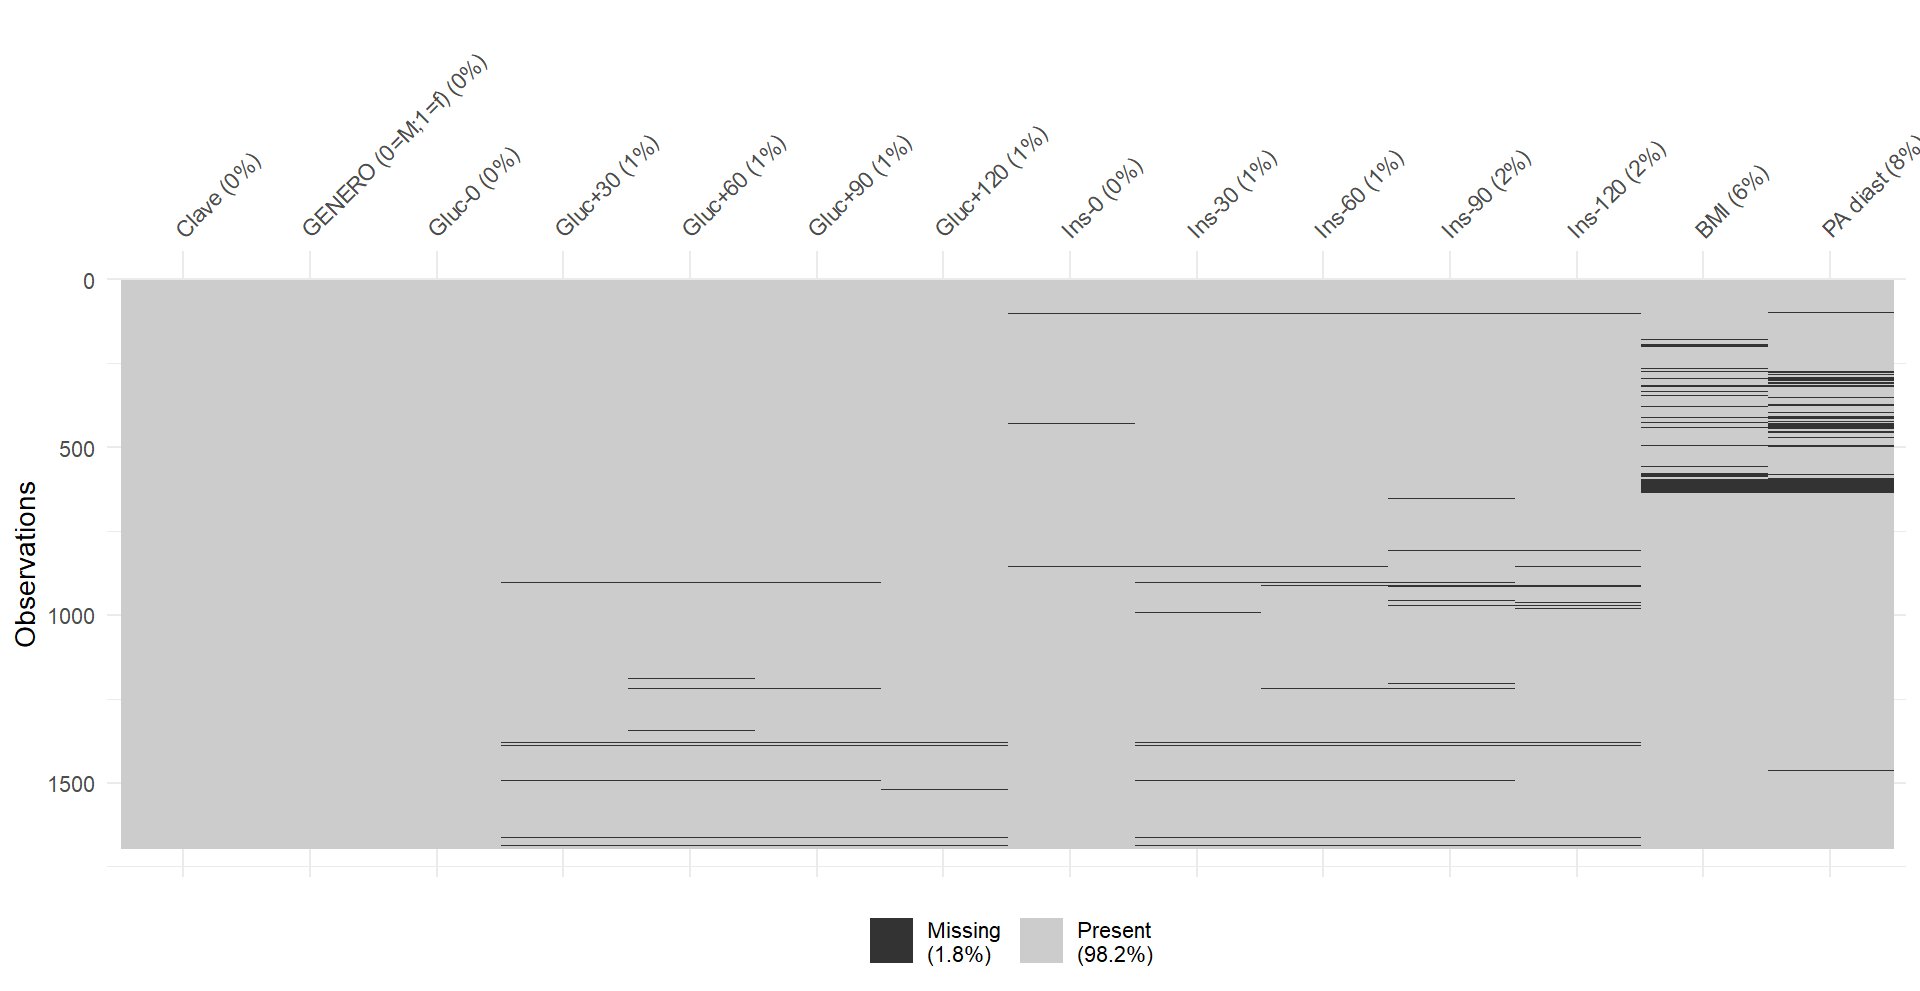
\includegraphics[width = 0.8 \textwidth, height = 6 cm]{Imagenes/datosFaltantes.png}
    \caption{Figura ilustrativa de los datos faltantes en la base de datos.}
    \label{fig:Nas}
\end{figure}

Para medir el nivel de datos faltantes de cada variable se toma la proporción de número de datos faltantes con respecto al total de datos. En el Cuadro \ref{tab:PorcentajeNA} se muestra el porcentaje de NA's de correspondiente a cada variable. Afortunadamente, esta cantidad no es mayor al $8 \%$; en casi todas las variables con datos faltantes esta cantidad es menor al $3\%$. 

\begin{table}[H]
\centering
\begin{tabular}{||c|c||c|c||}
\hline\hline
\textbf{Variable} & \textbf{\% de NA} & \textbf{Variable} & \textbf{\% de NA} \\ \hline\hline
PA diast          & 7.71950501        & BMI               & 6.01060695        \\ \hline
Ins-90            & 2.47495580        & Ins-120           & 2.23924573        \\ \hline
Ins-60            & 1.47318798        & Glu-90            & 1.41426046        \\ \hline
Glu-60            & 1.11962286        & Ins-30            & 1.06069534        \\ \hline
Glu-30            & 0.94284031        & Glu-120           & 0.64820271        \\ \hline
Ins-0             & 0.17678256        & -                 & -       \\ \hline\hline
\end{tabular}
\caption{Porcentaje de datos faltantes de cada variable.}
\label{tab:PorcentajeNA}
\end{table}

Considerando que el modelo estará especializado para su uso en el área médica y que la cantidad de datos faltantes no es excesiva, es preferible eliminar los individuos que contengan alguna covariable con valores faltantes (NA). Esto se debe a que utilizar técnicas de imputación puede alterar las relaciones estadísticas originales entre variables, afectando la capacidad del modelo para hacer inferencias válidas. En aplicaciones médicas, donde las decisiones basadas en el modelo pueden tener consecuencias significativas para la salud del paciente, es crucial mantener la precisión de estas inferencias. Además, la imputación puede distorsionar los patrones subyacentes en los datos, especialmente en conjuntos de datos médicos, donde las relaciones entre variables pueden ser complejas y no lineales, lo que puede llevar a modelos que no reflejen adecuadamente la realidad clínica.

\begin{figure}[H]
 \centering
  \subfloat[Mujeres]{
   \label{DatosFMu}
    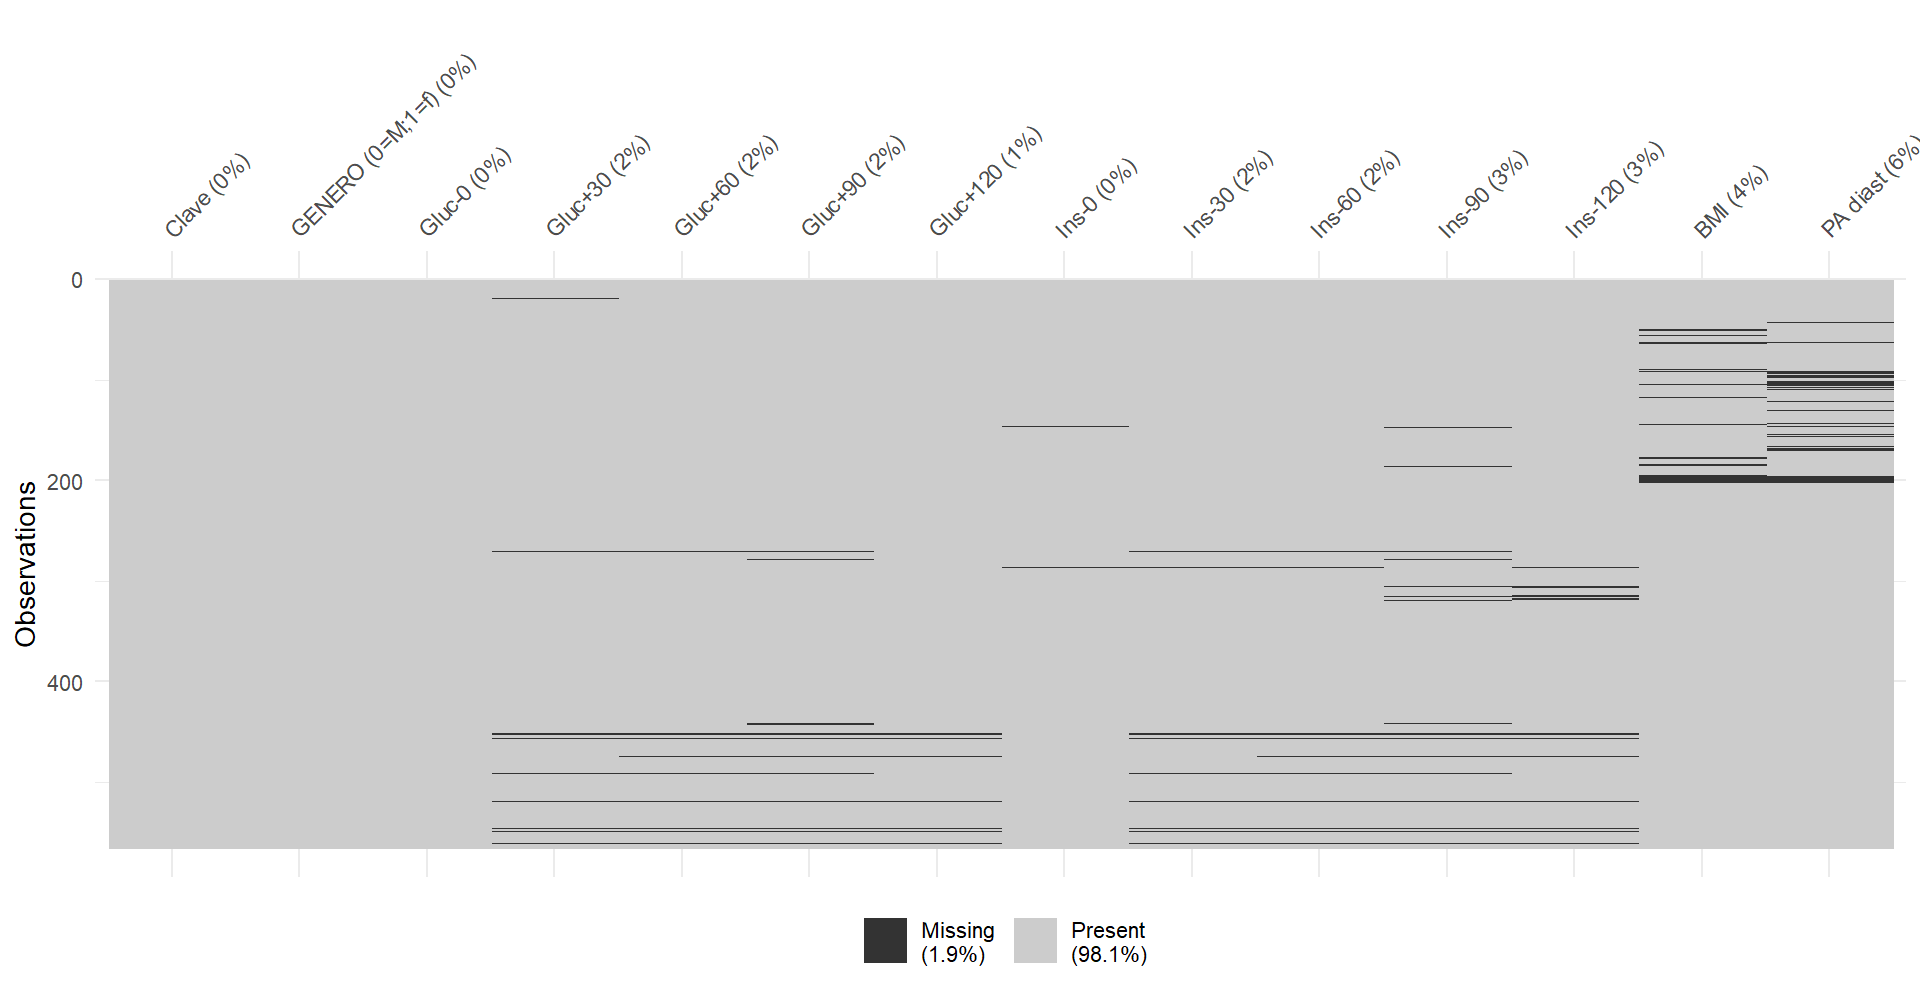
\includegraphics[width=0.45\textwidth]{Imagenes/datosFaltantesMujeres.png}}
  \subfloat[Hombres]{
   \label{Datos}
    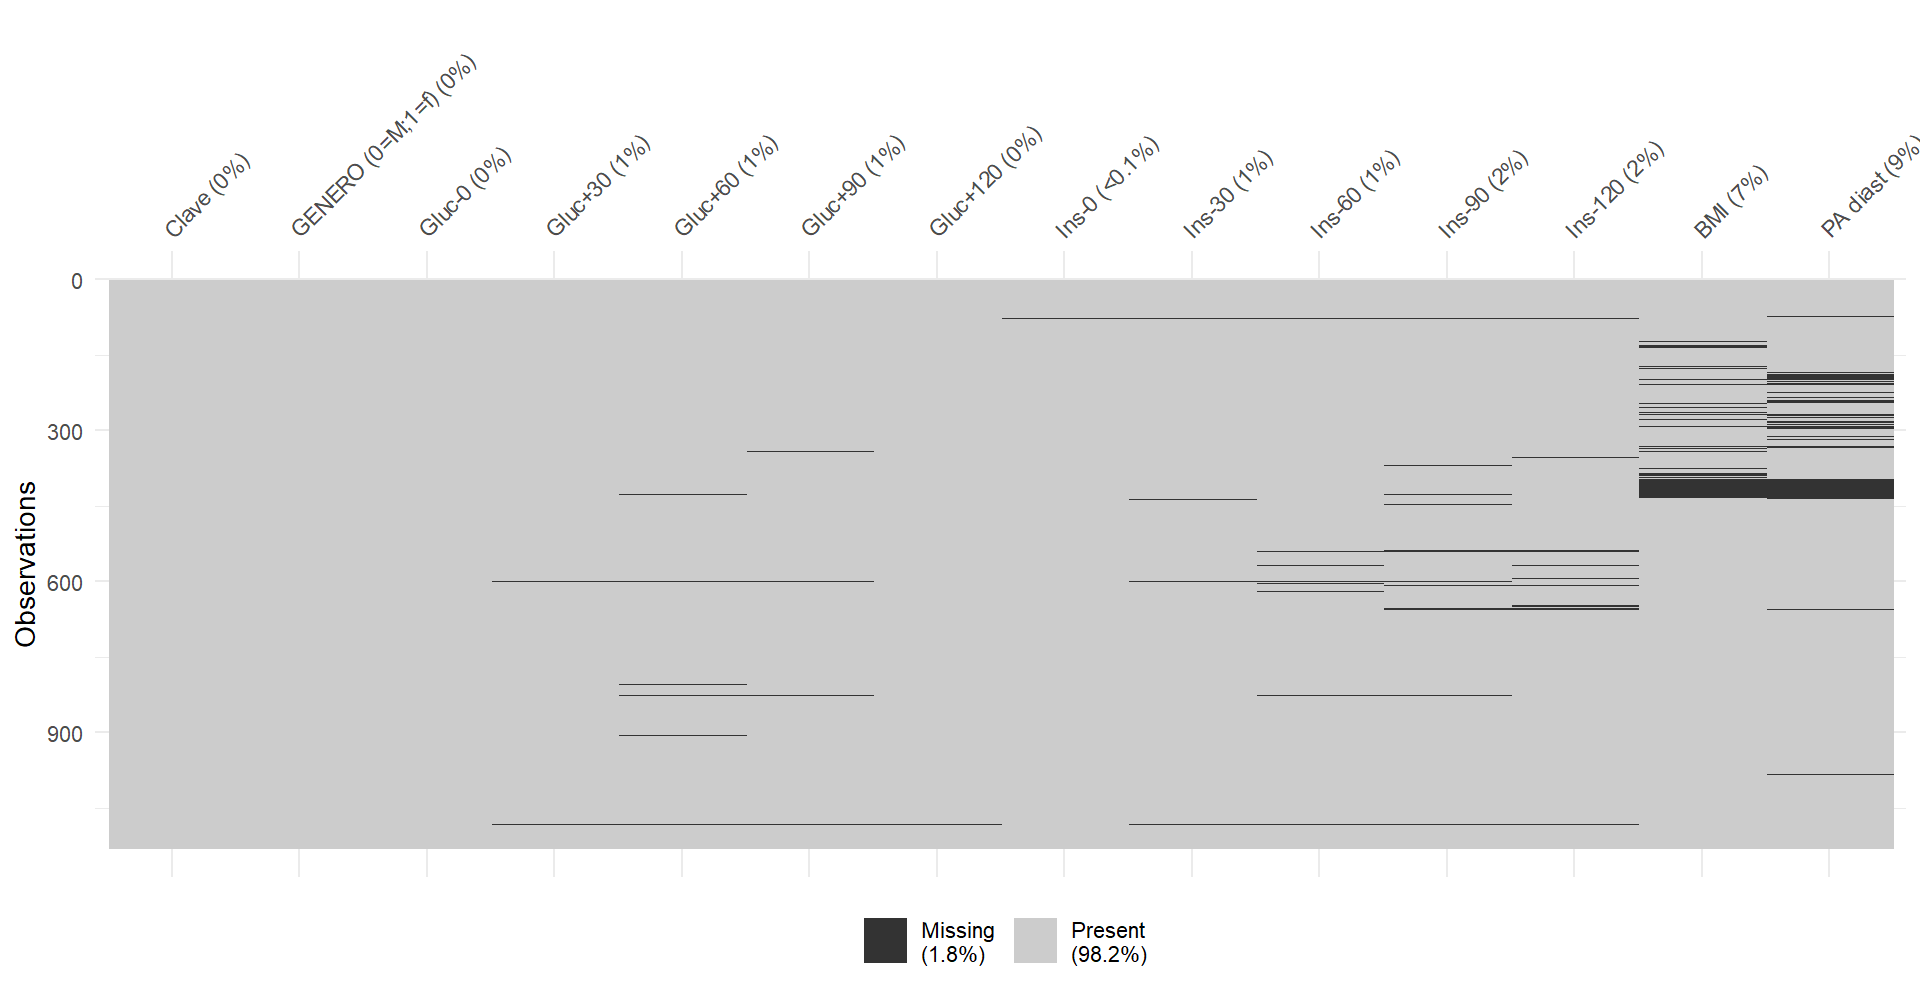
\includegraphics[width=0.45\textwidth]{Imagenes/datosFaltantesHombres.png}}
    \caption{Visualización de datos faltantes por género.}
    \label{fig:FaltantesGen}
\end{figure}

En la Figura \ref{fig:FaltantesGen}, se muestran los datos faltantes de acuerdo al género. En ambos géneros, las principales variables con datos faltantes son la presión diastólica y el índice de masa corporal. Sin embargo, la base de datos está desbalanceada en términos de género, con un total de $1131$ mujeres y $566$ hombres. Tener una base de datos desbalanceada puede presentar varias desventajas cuando se quieren implementar modelos por género. Como por ejemplo, puede causar que el modelo favorezca al grupo mayoritario, es decir, las predicciones y las inferencias serán más precisas para las mujeres en este caso, mientras que los hombres podrían no ser representados adecuadamente.

Después de remover los individuos que contienen alguna covariable con datos faltantes, la base de datos cuenta con un total de $1454$ individuos, de los cuales $956$ son mujeres y $498$ son hombres. Con este conjunto de datos se desarrollarán tres modelos: uno para la población en conjunto y dos modelos separados por género.

%%%%%%%%%%%%%%%%%%%%%%%%%%%%%%%%%%%%%%%%%%%%%%%%%%%%%%%%%%%%%%%%%%%%%
%%%%%%%%%%%%%%%%% 
%%%%%%%%%%%%%%%%%%%%%%%%%%%%%%%%%%%%%%%%%%%%%%%%%%%%%%%%%%%%%%%%%%%%%

\section{Visualización de Dependencias}

En algunas de las siguientes subsecciones se incluyen algunos otros estudios exploratorios. Por claridad y para hacer énfasis en su importancia, se decidió poner dichos análisis en subsecciones separadas. Para comenzar a analizar las dependencias entre las covariables, la Figura \ref{fig:corrSWE} presenta un mapa de calor elaborado con la matriz de correlación de Schweizer y Wolff, mientras que la Figura \ref{fig:corSpe} muestra un mapa de calor basado en la matriz de correlación de Spearman. Es importante recordar que el coeficiente de Spearman proporciona información sobre la dirección de la dependencia entre las variables. En la Figura \ref{fig:corSpe}, el mapa de calor revela que todas las dependencias identificadas son crecientes o positivas.

Adicionalmente, en el mapa de calor de la correlación de Schweizer y Wolff, se observa una dependencia significativa entre las mediciones de la curva de glucosa. Sin embargo, en cuanto a las mediciones de insulina, aunque las dependencias no son tan fuertes como las observadas en las variables de glucosa, siguen siendo considerables. Como se mencionó en el Capítulo \ref{insulina}, los niveles de insulina y glucosa en sangre durante la prueba oral de glucosa no son independientes. Sin embargo, las dependencias no son tan marcadas, aunque sí están presentes. 

\begin{figure}[H]
    \centering
    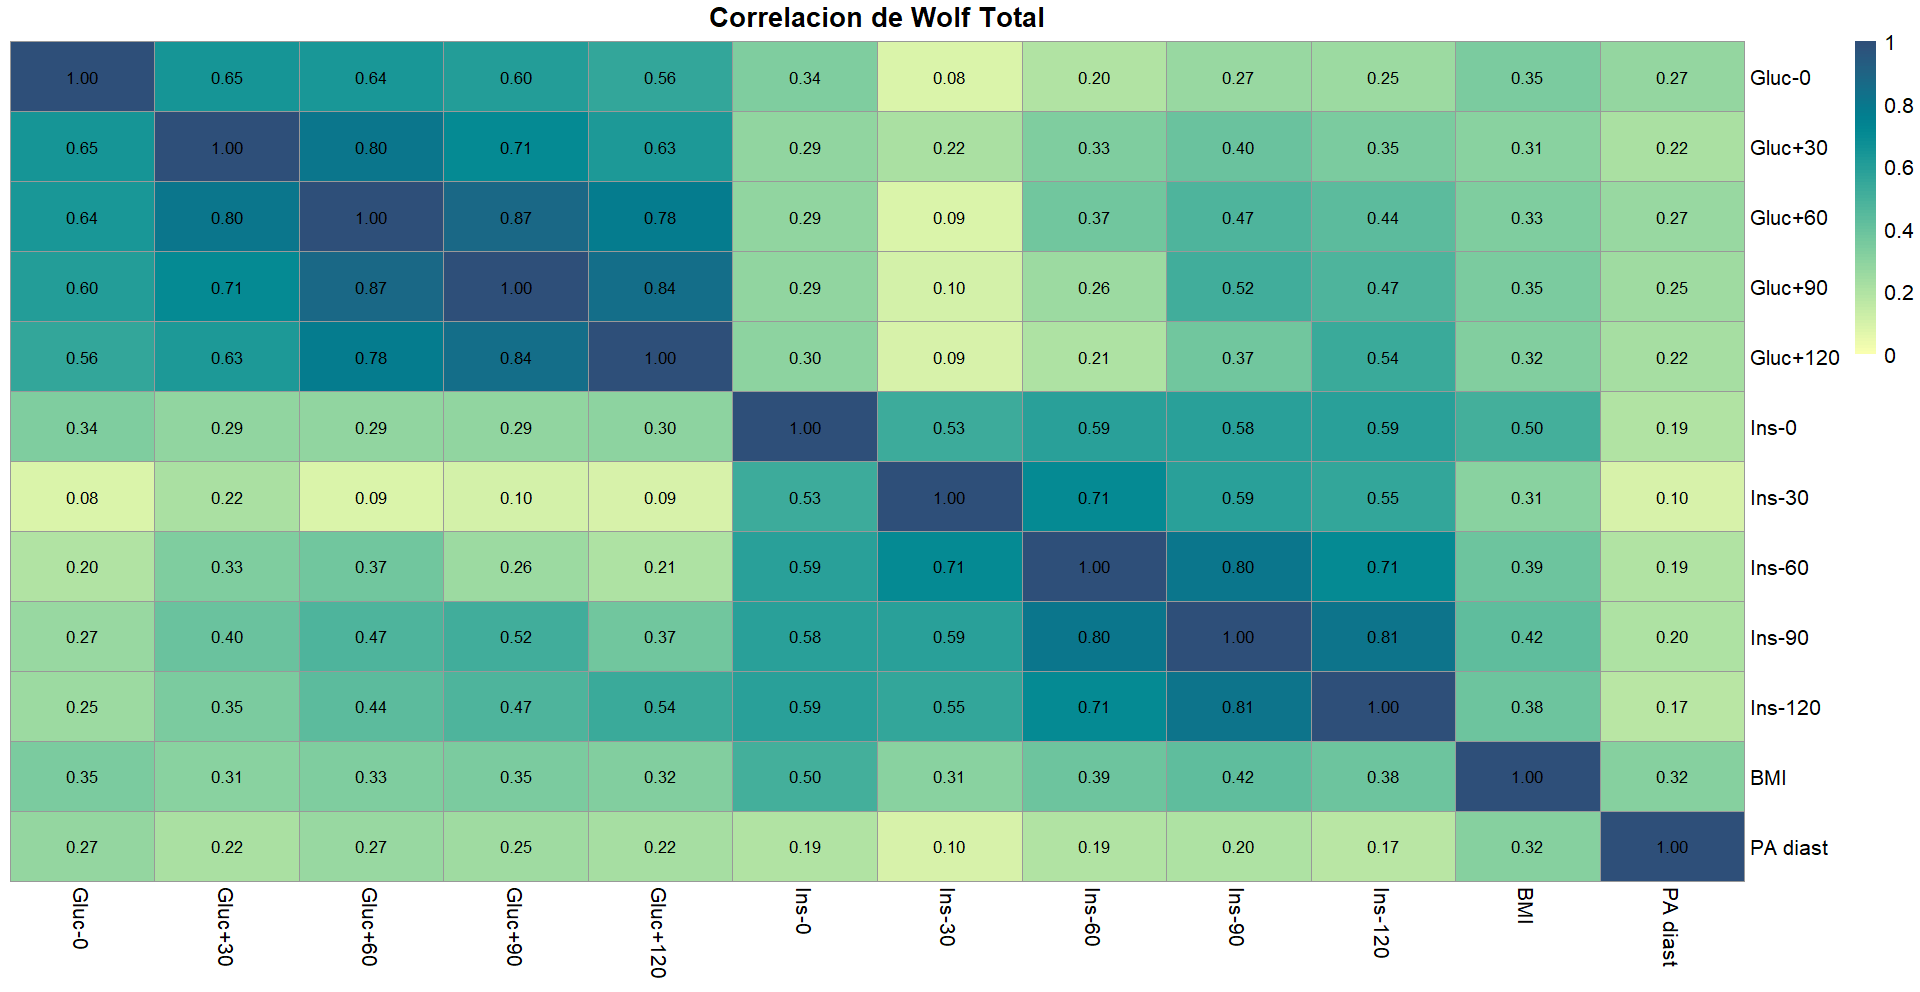
\includegraphics[width = 0.9 \textwidth]{Imagenes/corWolfTotal.png}
    \caption{Heatmap de las covariables numéricas con la correlación de Schweizer y Wolff.}
    \label{fig:corrSWE}
\end{figure}

\begin{figure}[H]
    \centering
    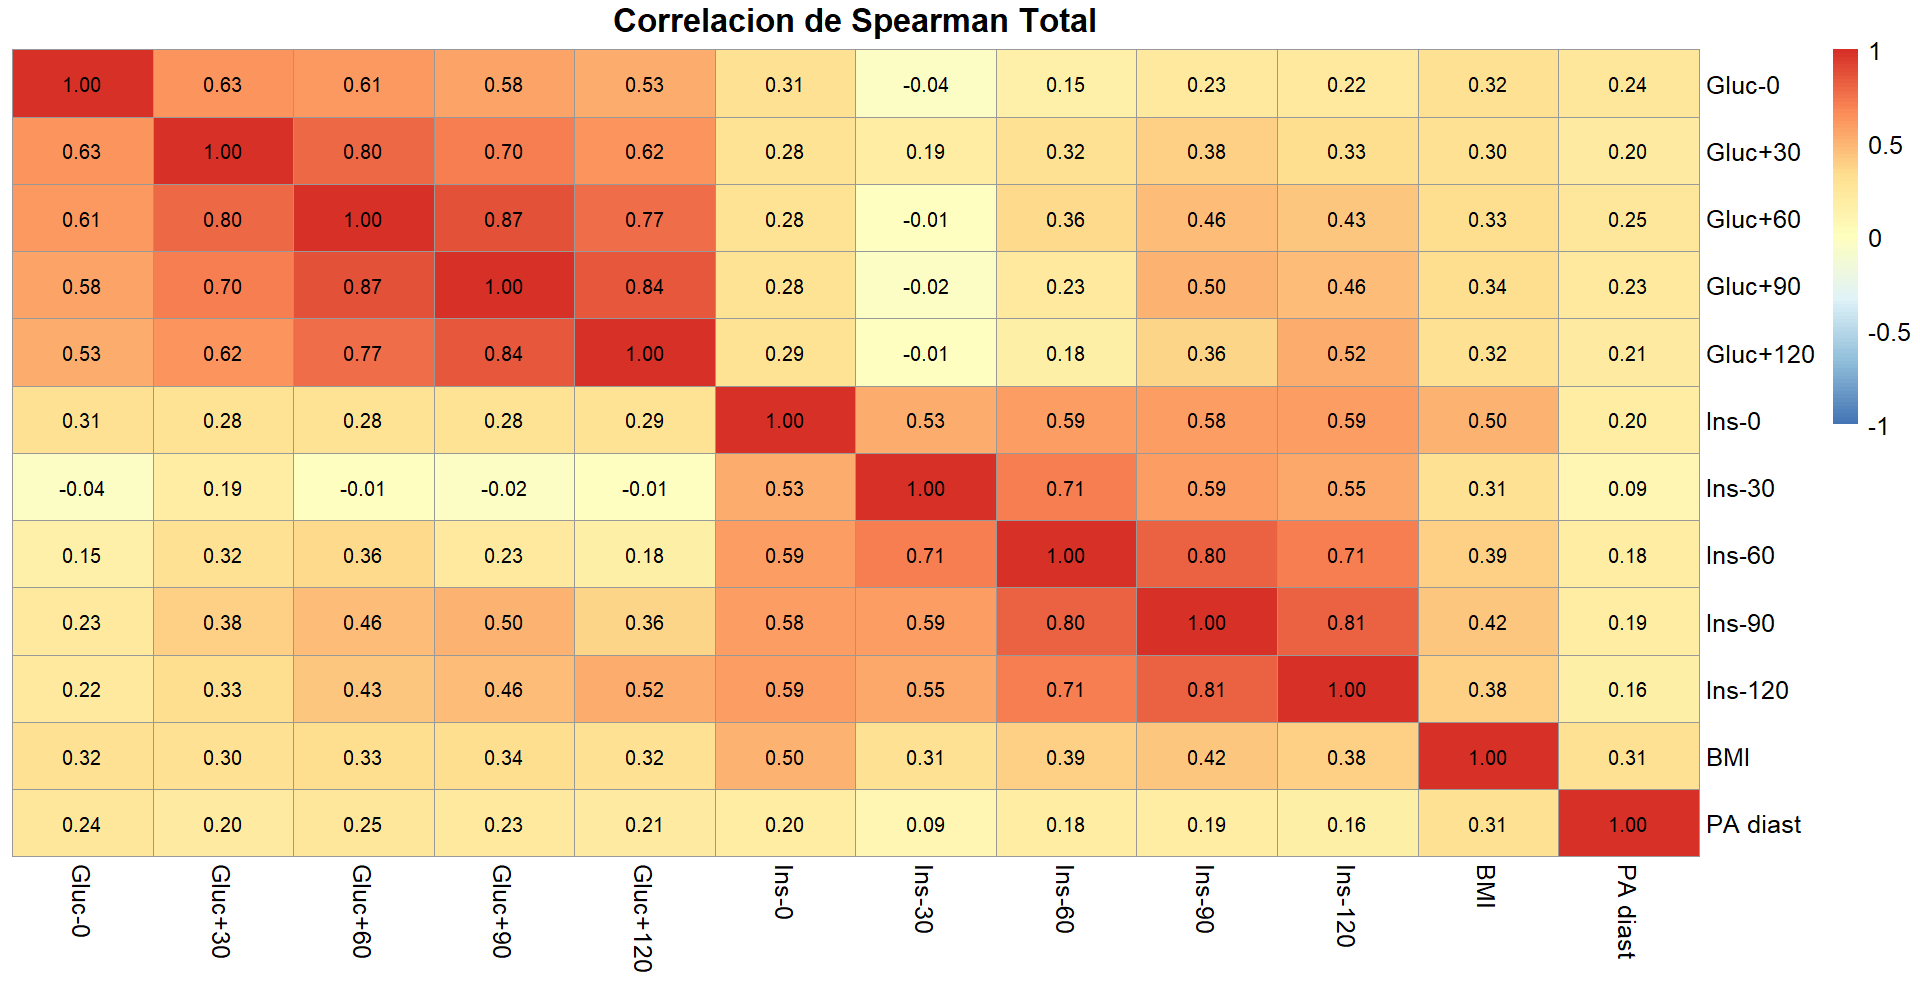
\includegraphics[width = 0.9 \textwidth]{Imagenes/corSperTotal.png}
    \caption{Heatmap de las covariables numéricas con la correlación de Spearman.}
    \label{fig:corSpe}
\end{figure}

El objetivo es utilizar las cópulas para modelar adecuadamente las interacciones entre la glucosa y la insulina, ya que estas interacciones son fundamentales para inferir el estado de las células beta del páncreas y proporcionar una alerta adecuada sobre la enfermedad. Al capturar la naturaleza compleja y no lineal de estas dependencias, el uso de cópulas permite una representación más precisa de las relaciones subyacentes, mejorando así la capacidad de detección temprana y el manejo de enfermedades como la diabetes.


\begin{figure}[H]
 \centering
  \subfloat[Mujeres]{
   \label{CorWolfMu}
    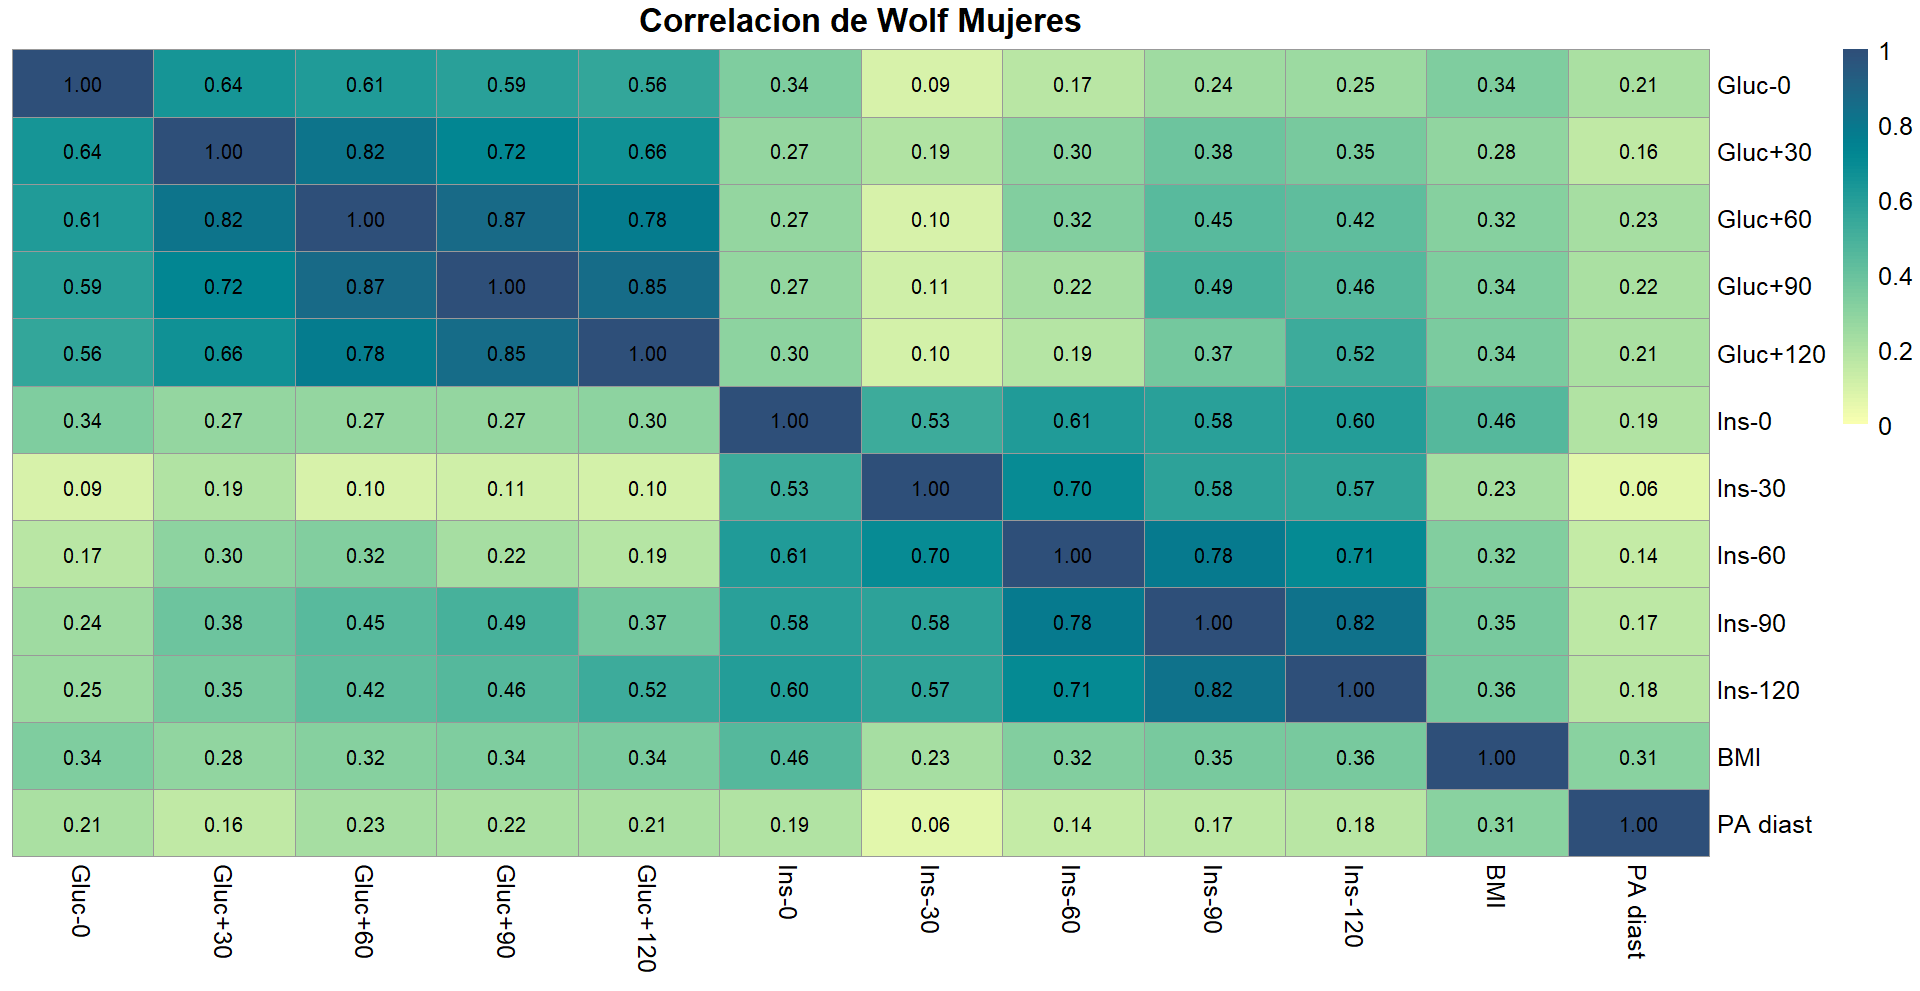
\includegraphics[width=0.48\textwidth]{Imagenes/corWolfMuj.png}}
  \subfloat[Hombres]{
   \label{CorWolfHom}
    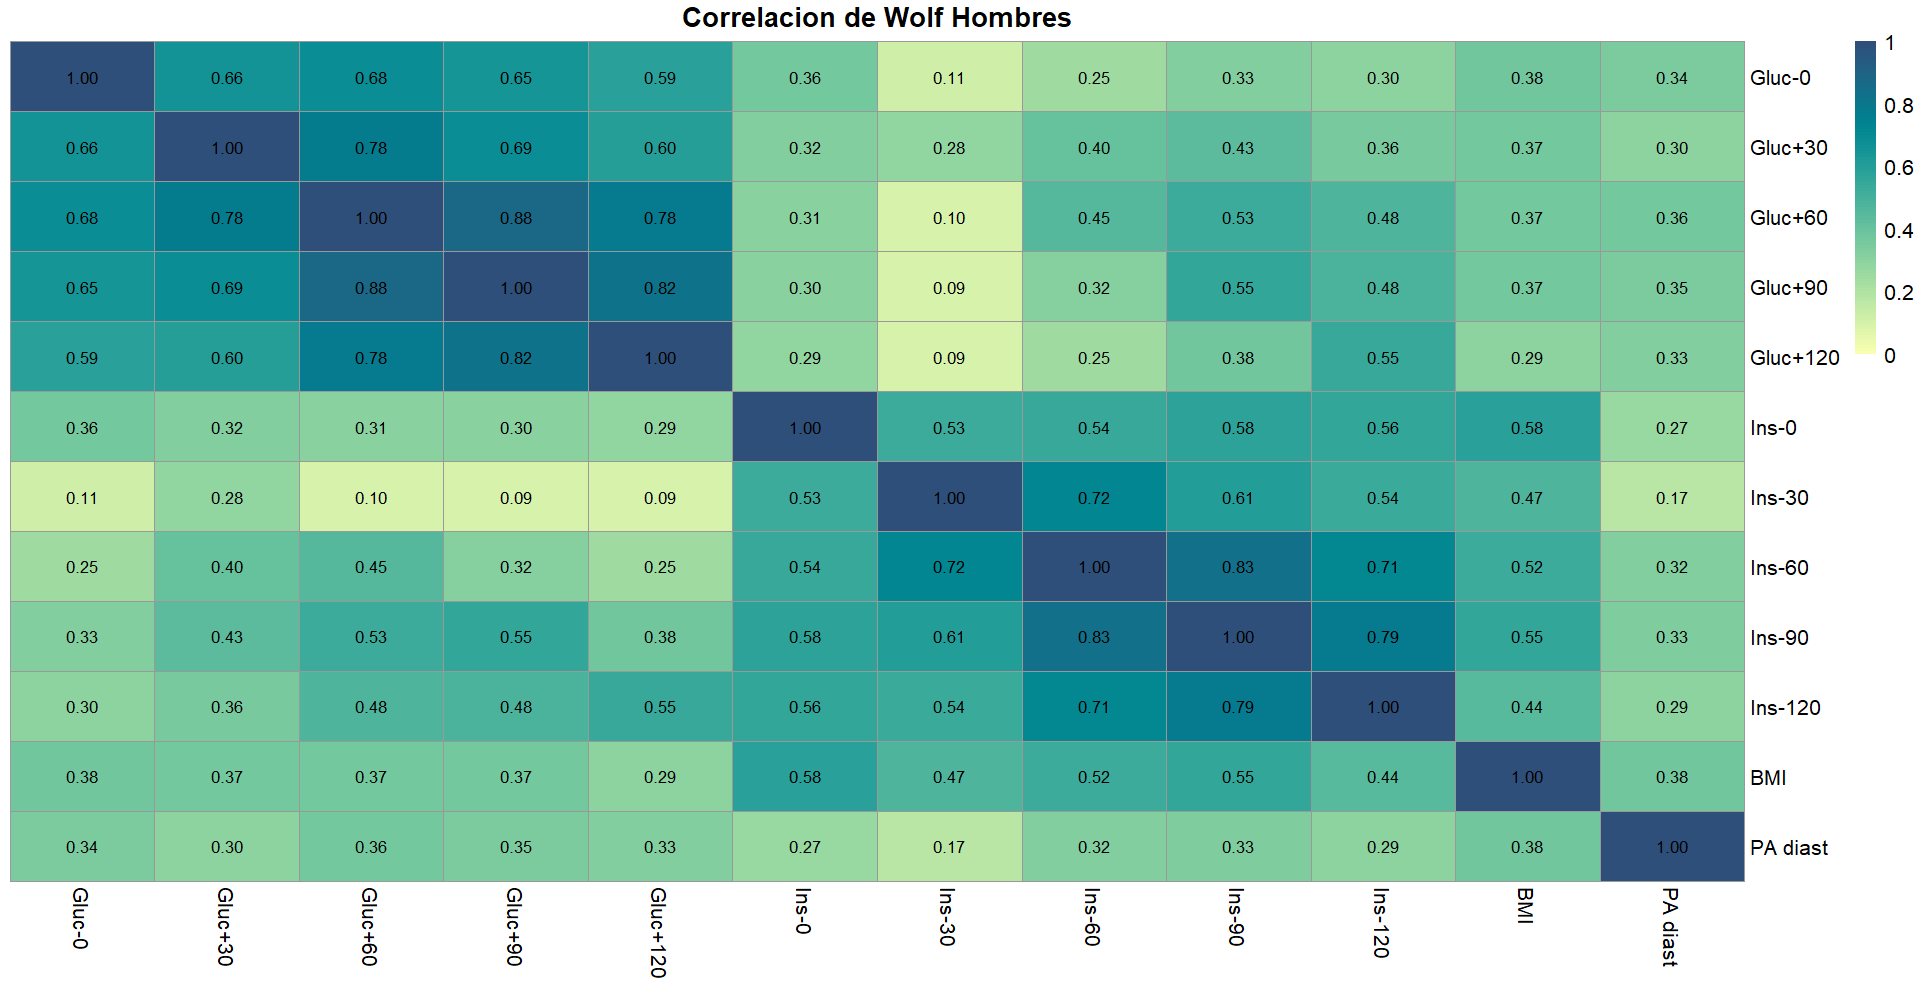
\includegraphics[width=0.48\textwidth]{Imagenes/corWolfHom.png}}
    \caption{Visualización de heatmaps por Género.}
    \label{fig:CorWolfGen}
\end{figure}

En la Figura \ref{fig:CorWolfGen}, se presentan los mapas de calor de la matriz de correlación de Wolf, desglosados por género. Sin embargo, no se aprecian diferencias significativas. Aunque algunas relaciones entre glucosa e insulina son más fuertes en mujeres que en hombres. Esto podría deberse al desbalance en la cantidad de datos disponibles, más que a una diferencia intrínseca relacionada con el género. Se espera que el modelo basado en cópulas sea capaz de discernir estas diferencias y proporcionar una interpretación más precisa de las dependencias entre las variables, tomando en cuenta tanto el posible desbalance de datos como las variaciones debidas al género.


%%%%%%%%%%%%%%%%%%%%%%%%%%%%%%%%%%%%%%%%%%%%%%%%%%%%%%%%5
%%%%%%%%%%%%%%%%%%%%%%%%%%%%%%%%%%%%%%%%%%%%%%%%%%%%%%%%%

 \subsection{Clasificación de Variables}\label{ClasificaVar}

\begin{table}[H]
    \centering
    \begin{tabular}{||c|c||}
    \hline\hline
    \textbf{Rango}                  & \textbf{Clasificación} \\ \hline\hline
    $ BMI < 25$            & Normal                 \\ \hline
    $25\leq BMI<30$                 & Sobrepeso              \\ \hline
    $ BMI > 35$               & Obesidad       \\ \hline\hline
\end{tabular}
\caption{Clasificación del grado de obesidad de acuerdo al IBM.}
\label{tab:clasBMI}
\end{table}

A partir de las variables que se tienen se pueden crear otras variables. A continuación, se describe las nuevas variables introducidas.  En función del índice de masa corporal, se introdujeron los grados de obesidad como la Dra. Monroy lo sugirió. En el Cuadro \ref{tab:clasBMI} se marca esta clasificación.
Como breve resumen, se clasificaron $375$ como normal, $594$ con sobrepeso, $397$ con obesidad $1$, $158$ con obesidad $2$ y $71$ con obesidad $3$. 
 


En base a las mediciones en el tiempo de las concentraciones de glucosa se puede hacer una clasificación. En el Cuadro \ref{tab:diagnostico} se puede distinguir estas clasificaciones, las cuales fueron hechas de acuerdo a otra sugerencia de la Dra. Monroy. Como resultado de esta división, se encuentran $82$ diabéticos, $567$ con prediabéticos y $916$ individuos en un estado normal.

\begin{table}[H]
\centering
\begin{tabular}{||c|c||}
\hline\hline
\textbf{Criterio}                       & \textbf{Diagnóstico} \\ \hline\hline
$G_0 \leq100$ y $G_{120} \leq 140$   & Normal               \\ \hline
$G_{0} > 100$ y $G_{0} < 126$  & Prediabetes          \\ \hline
$G_{120} \geq 140$ y $G_{120} < 200$ & Prediabetes          \\ \hline
$G_0 \geq 126$                     & Diabetes             \\ \hline
$G_{120} \geq 200$                  & Diabetes             \\ \hline
En otro caso                            & Incierto              \\ \hline\hline
\end{tabular}
\caption{Diagnóstico de acuerdo a la curva de Glucosa.}
\label{tab:diagnostico}
\end{table}

Con el objetivo de visualizar el procesamiento de glucosa e insulina de acuerdo al índice de masa corporal, en la Figura \ref{fig:CurvasGluIBM} se muestran las curvas de glucosa clasificadas según la categoría de índice de masa corporal. Algunos aspectos destacables son los siguientes: 

\begin{figure}[H]
    \centering
    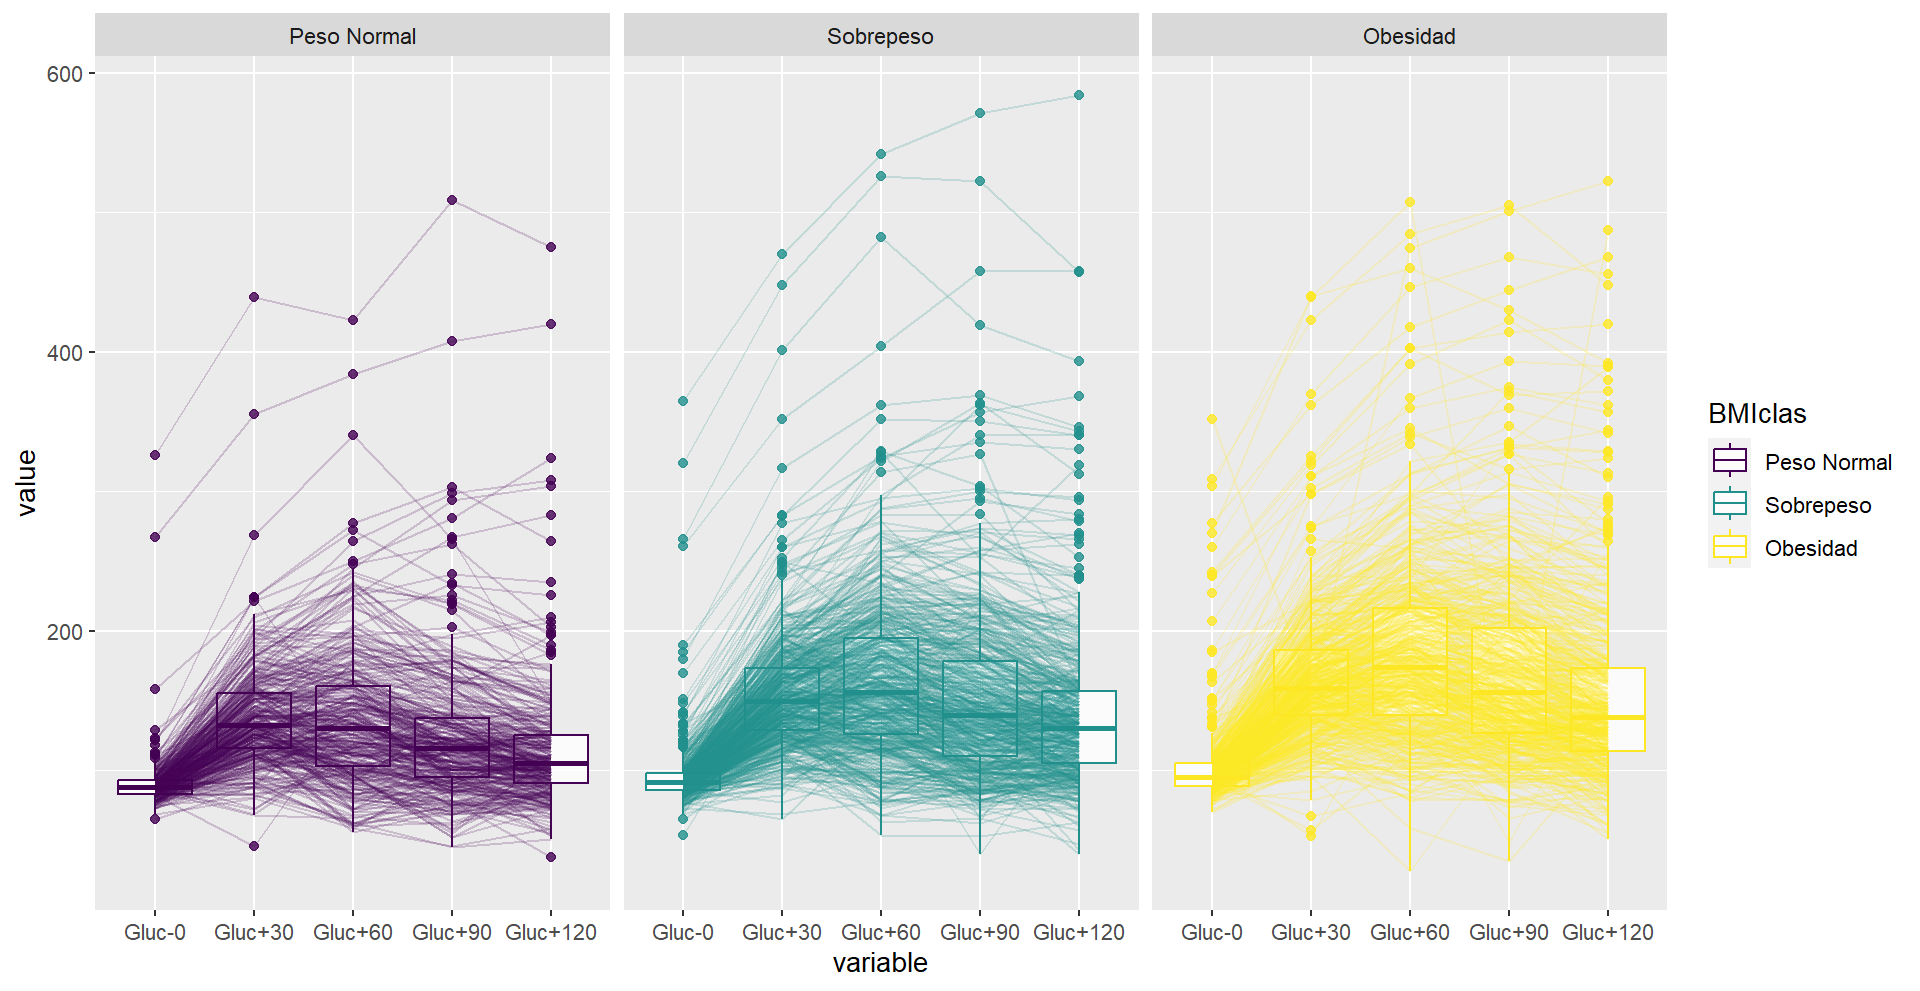
\includegraphics[width = 0.98 \textwidth]{Imagenes/gluCurvasBMI.png}
    \caption{Curvas de glucosa acuerdo al índice de masa corporal.}
    \label{fig:CurvasGluIBM}
\end{figure}

\begin{itemize}
    \item Los pacientes con peso normal mayoritariamente presentan curvas de glucosa dentro de los rangos esperados, como se observa en los boxplots a los tiempos $0$ y $120$, donde los valores son más bajos en comparación con pacientes con sobrepeso u obesidad. Sin embargo, es importante destacar que tener un peso normal no garantiza estar libre de riesgos, ya que también se pueden observar curvas con niveles elevados de glucosa.

    \item Los pacientes con sobrepeso muestran mayor variabilidad, con rangos más altos, especialmente a los minutos $90$ y $120$. Esto se puede observar en los boxplots correspondientes a eso minutos. En este grupo es donde se observa el paciente con la curva de glucosa más alta, lo cual podría indicar estrés en las células beta del páncreas.

    \item Los individuos con obesidad presentan curvas con rangos más altos en los minutos $60$, $90$ y $120$, como se refleja en sus respectivos boxplots.  Sin embargo, también se observa que hay más individuos dentro de este grupo que muestran curvas con niveles muy elevados de glucosa pero también se encuentran individuos con curvas en rangos normales, lo cual indica que la obesidad es un factor influyente pero no determinante.
\end{itemize}

Como conclusión de estas observaciones, se espera que las cópulas puedan capturar esta relación, ya que el índice de masa corporal influye en el diagnóstico de la diabetes, aunque no de manera determinante. Si bien los individuos con sobrepeso u obesidad tienden a mostrar niveles más altos de glucosa e insulina, también se observa una considerable variabilidad dentro de estos grupos. Esto sugiere que la obesidad es un factor importante pero no único en la predisposición a la diabetes.


\begin{figure}[H]
    \centering
    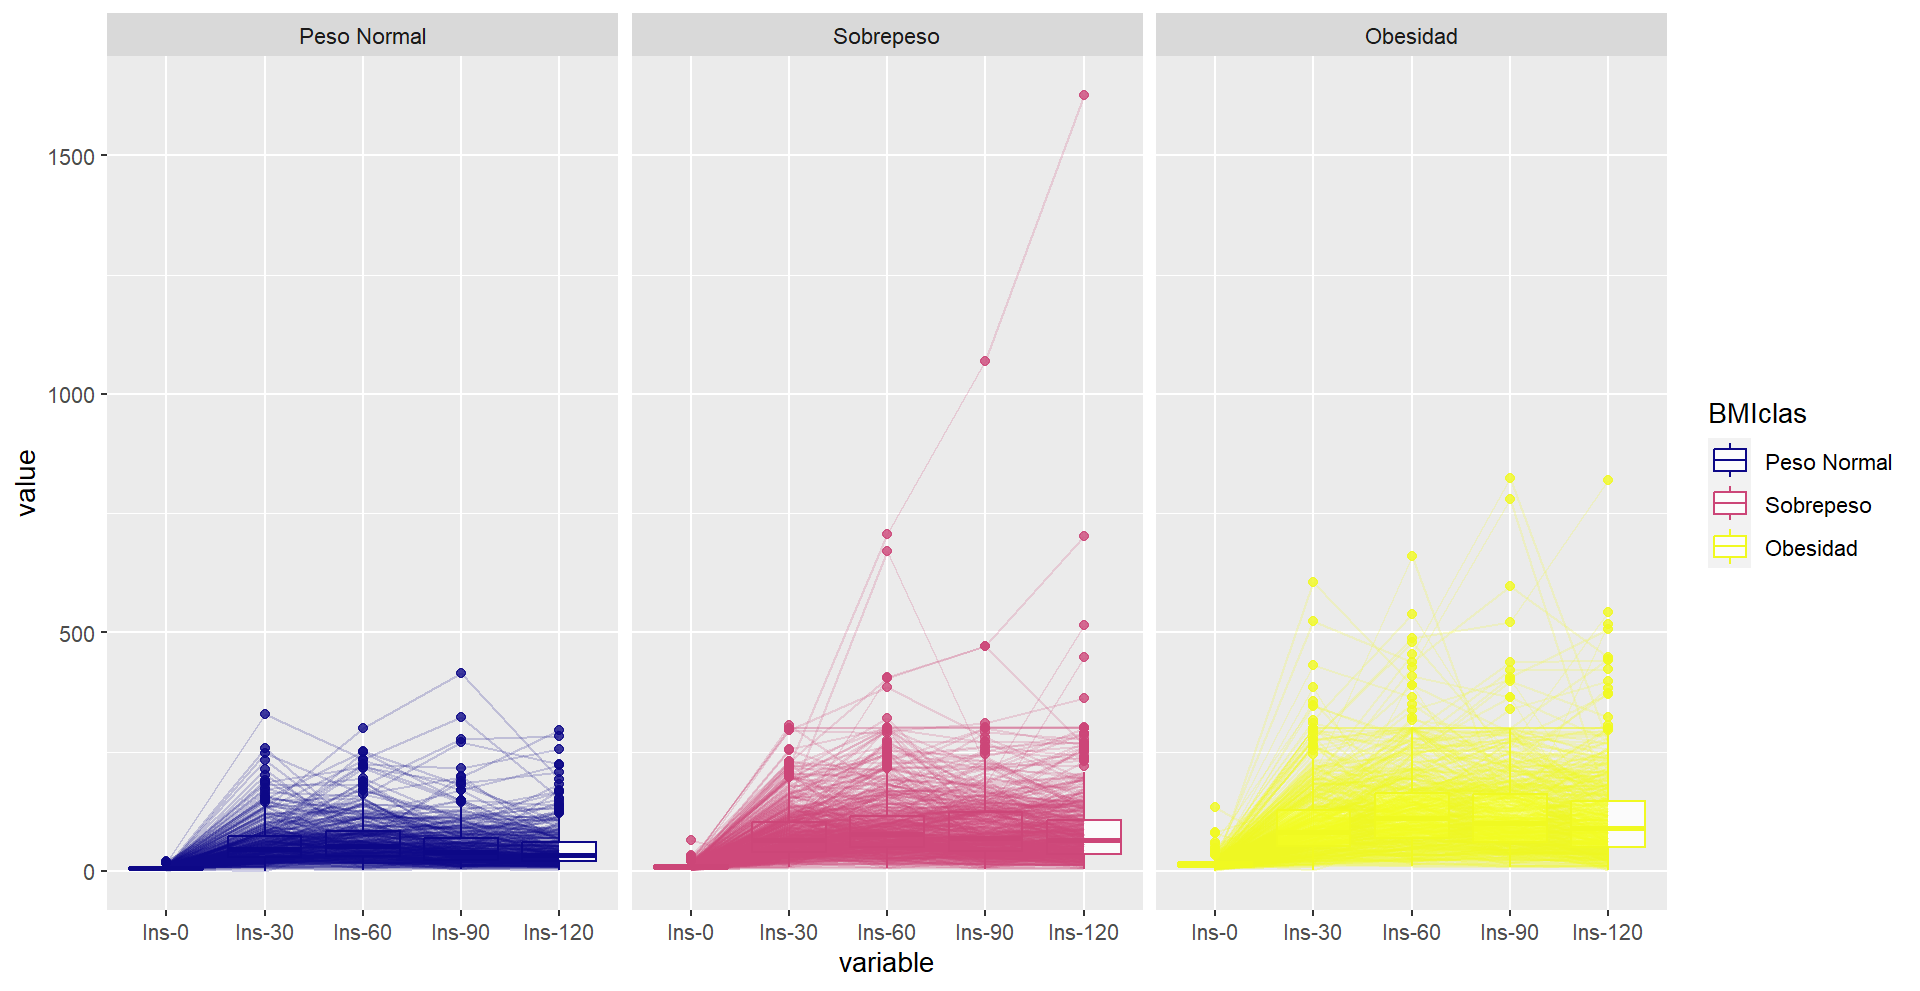
\includegraphics[width = 0.9 \textwidth]{Imagenes/insCurvasBMI.png}
    \caption{Curvas de insulina de acuerdo al índice de masa corporal.}
    \label{fig:CurvasInsIBM}
\end{figure}

Para continuar con este análisis por índice de masa corporal, en la Figura \ref{fig:CurvasInsIBM} se muestran las curvas de respuesta de la insulina. Los elementos destacables son:

\begin{itemize}
    \item  Las curvas correspondientes a pacientes con peso normal muestran un patrón generalmente cóncavo. Sin embargo, también se pueden observar casos donde la curva no sigue este patrón cóncavo tan pronunciado, sino que inicialmente es creciente y luego apenas decrece en los últimos minutos, lo cual podría indicar un inicio de falló en la efectividad de la insulina.

    \item Los pacientes con sobrepeso presentan curvas muy variadas. Algunos muestran la característica forma cóncavo, que es indicativa de una respuesta normal de la insulina. Sin embargo, también se observan curvas que parecen ser simplemente crecientes, lo cual sugiere una clara disfunción de las células beta del páncreas. Este patrón indica un inicio de fallo en la efectividad de la insulina, siendo un hallazgo preocupante en pacientes con sobrepeso.

    \item Los pacientes con obesidad presentan curvas que sugieren resistencia a la insulina en diferentes grados. Algunas curvas muestran un descenso en los últimos instantes, lo cual indica que la resistencia a la insulina podría ser reversible en cierta medida. Sin embargo, también se observan curvas donde la producción de insulina es prácticamente nula. Esto sugiere un claro agotamiento de las células beta del páncreas, lo cual es preocupante y podría indicar un deterioro avanzado en la capacidad del cuerpo para regular los niveles de glucosa.
    \end{itemize}

Como se pudo observar anteriormente, la relación entre la glucosa y la insulina no es trivial de modelar. En la siguiente sección, se hará más énfasis en esta relación y en los momentos cruciales para identificar y alertar antes de que esta enfermedad sea irreversible.

%%%%%%%%%%%%%%%%%%%%%%%%%%%%%%%%%%%%%%%%%%%%%%%%%%%%%%%%%%%%
%%%%%%%%%%%%% Resultados de Boxplot Funcioles %%%%%%%%%%%%%%
%%%%%%%%%%%%%%%%%%%%%%%%%%%%%%%%%%%%%%%%%%%%%%%%%%%%%%%%%%%%

\section{Resultados de Boxplot Funcionales}

Según el artículo `\textit{Gender differences in glucose homeostasis and diabete}' \cite{GenderDifferences2018}, existen diferencias notables en el proceso de homeostasis de la glucosa entre hombres y mujeres que pueden ser relevantes durante el modelado. Esto adquiere importancia porque el propósito es desarrollar dos modelos distintos para predecir la resistencia a la insulina. Por ejemplo, se destaca que las mujeres muestran niveles más bajos de glucosa plasmática en ayunas y niveles más altos de glucosa plasmática a las 2 horas en comparación con los hombres.

\subsection{Construcción de un Boxplot Funcional}

Antes del comenzar el análisis gráfico, se presentará una breve descripción de la construcción de los boxplots funcionales para mejorar la interpretación de la gráfica para algo más detallada se sugiera consultar el artículo `\textit{Functional Boxplots}' \cite{boxplotFun}. La construcción de los boxplots funcionales sigue un proceso similar al de los boxplots clásicos, pero utiliza una medida de profundidad como las descritas en el Capítulo \ref{RegCuanDatosFun}:

\begin{figure}[H]
    \centering
    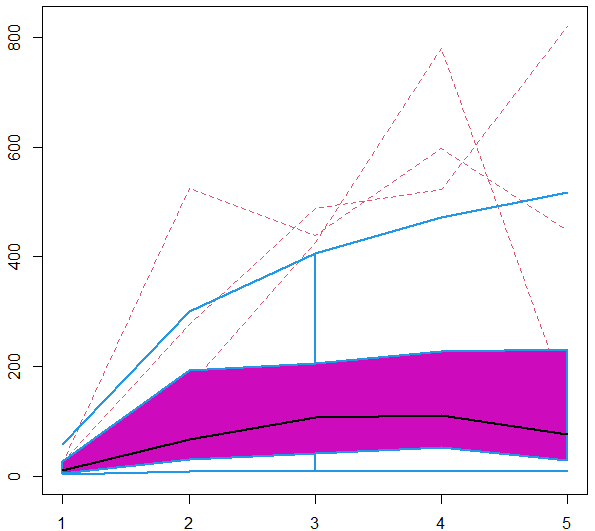
\includegraphics[width=0.5\linewidth]{Imagenes/partes.png}
    \caption{Parte de un Boxplot Funcional.}
    \label{fig:bfpartes}
\end{figure}

\begin{itemize}
    \item \textbf{Curva más profunda}. Se identifica la curva central o más profunda de las funciones empleando la medida de profundidad, que es la región donde se encuentra la mitad central de las curvas de datos, esta se muestra en negro en la Figura \ref{fig:bfpartes}. La curva mediana es una estadística robusta para medir la centralidad de las funciones.

    \item \textbf{El envolvente o caja}. Esta región es análoga al rango intercuartílico en un boxplot tradicional, y proporciona una indicación útil de la dispersión del $50\%$ central de las curvas. Esta esta definida por

    \begin{equation}
        C_{0.5} = \left\{(t, x(t)): \min _{r=1, \ldots,\lceil n / 2\rceil} x_{[r]}(t) \leq x(t) \leq \max _{r=1, \ldots,\lceil n / 2\rceil} x_{[r]}(t)\right\},
    \end{equation}

    donde $n$ es total de datos, $ \left \lceil \frac{n}{2}\right \rceil$ es el entero no más grande que $n/2$ y a $C_{0.5}$ se le llama el envolvente del $50 \%$. Esta se muestra en lila en la Figura \ref{fig:bfpartes}.
    
    \item \textbf{Bigotes}. Estos son líneas verticales que se extienden desde la caja y representan el máximo envolvente del conjunto de datos, excepto los outliers. Se construyen extendiendo el criterio de $1.5$ veces el rango intercuartílico de un boxplot tradicional. Para ello, se infla el envolvente de $50\%$ multiplicando su rango por $1.5$. En la Figura \ref{fig:bfpartes}, corresponden a las lineas azules.

    \item \textbf{Outliers}. Cualquier curva que se encuentre por fuera de los bigotes es marcada como un outlier. Estas curvas están marcadas con lineas rojas punteadas en la Figura \ref{fig:bfpartes}.
\end{itemize}
%%%%%%%%%%%%%%%%%%%%%%%%%%%%%%%%%%%%%%%%%%%%%%%%%%%%%%%%%%
%%%%%%% Boxplot's Funcionales de Glucosa e Insulina %%%%%% 
%%%%%%%%%%%%%%%%%%%%%%%%%%%%%%%%%%%%%%%%%%%%%%%%%%%%%%%%%%

\subsection{Boxplot's funcionales para la Glucosa e Insulina}

A continuación, se llevará a cabo un análisis exploratorio para identificar elementos relevantes, como las diferencias en las formas o rangos de las curvas de glucosa e insulina entre los grupos de hombres y mujeres, así como los grupos definidos por las clasificaciones del prediagnóstico sugerido.



\begin{figure}[H]
 \centering
  \subfloat[Boxplot Funcional de glucosa]{
   \label{bfGluTotal}
    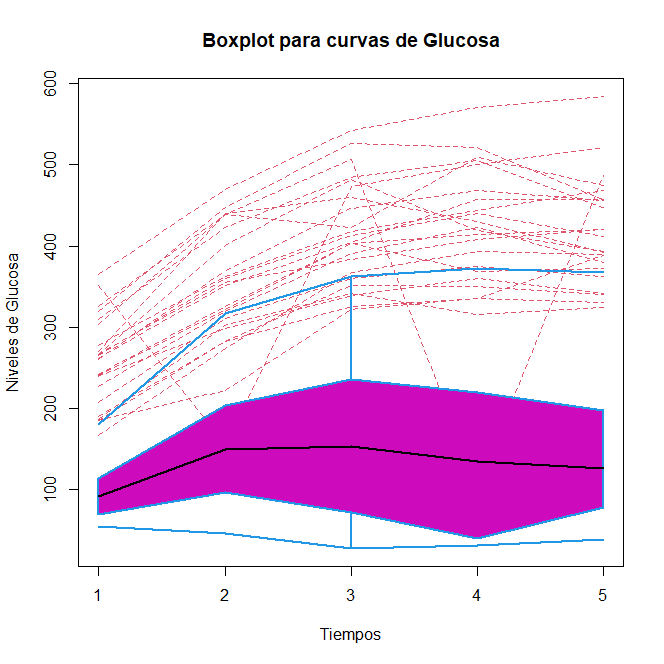
\includegraphics[width=0.47\textwidth]{img/bfTotalGlu.png}}
  \subfloat[Curvas de glucosa]{
   \label{dispGluTotal}
    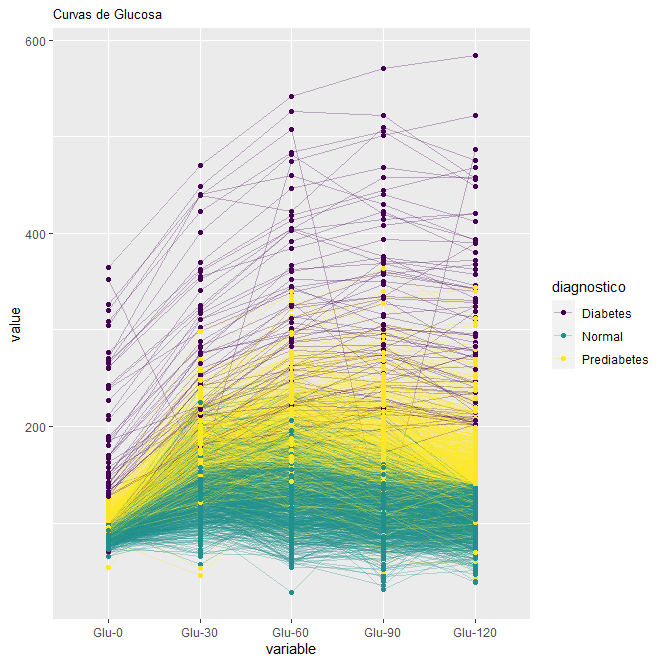
\includegraphics[width=0.47\textwidth]{img/disperGlu.png}}
    \caption{Gráficos de exploración de las curvas de glucosa.}
    \label{fig:glucosa}
\end{figure}


En la figura \ref{bfGluTotal} se presenta un boxplot funcional de las curvas de glucosa. El comportamiento de la curva mediana alcanza su punto máximo durante los primeros $60$ minutos y luego comienza a descender. Se observa que la mayoría de los datos atípicos corresponden al grupo de diabéticos, indicado en morado en la Figura \ref{dispGluTotal}. Además, se identifican algunos datos cuyas curvas parecen tener un patrón de subida, bajada y nueva subida, lo cual sugiere la posibilidad de errores de medición o que sugieren un error inherente. Otro aspecto destacable es la similitud entre las curvas correspondientes al tercer y primer cuartil, lo que sugiere una tendencia consistente en el procesamiento de la glucosa en sangre dentro de estos rangos.


\begin{figure}[H]
 \centering
  \subfloat[Boxplot Funcional de insulina]{
   \label{bfInsTotal}
    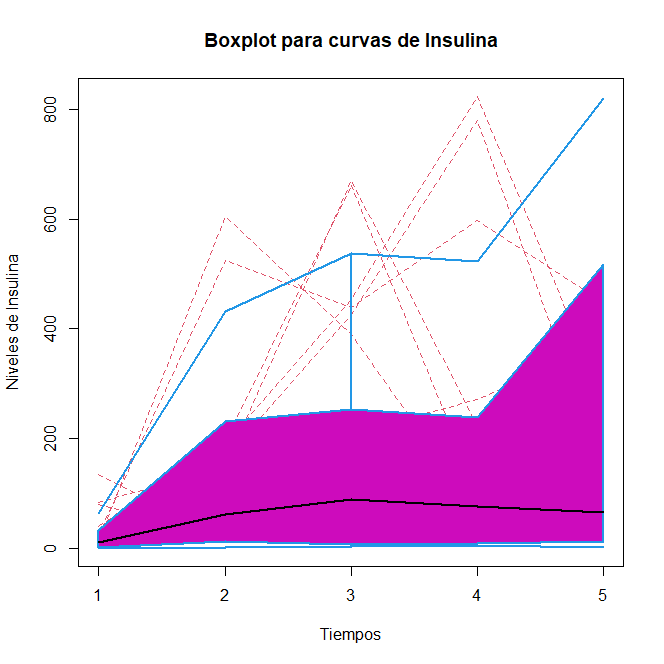
\includegraphics[width=0.47\textwidth]{img/bfTotalIns.png}}
  \subfloat[Curvas de insulina]{
   \label{dispInsTotal}
    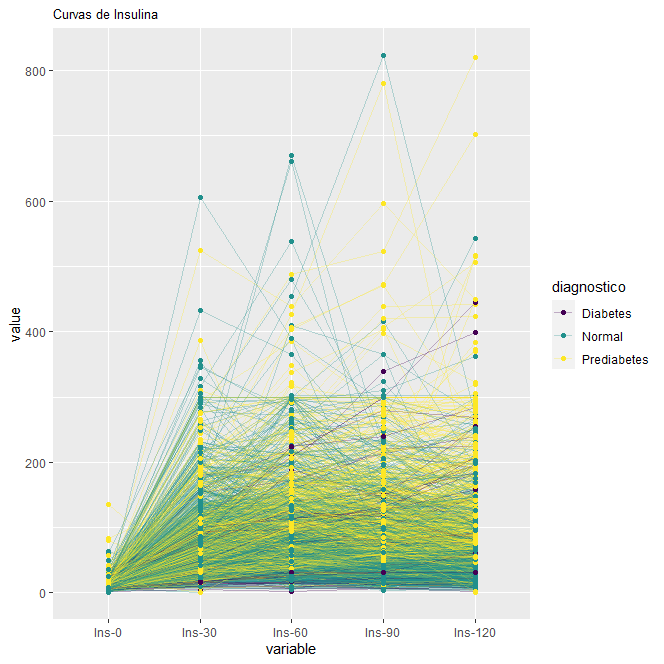
\includegraphics[width=0.47\textwidth]{img/dispeIns.png}}
    \caption{Gráficos de exploración de las curvas de insulina.}
    \label{fig:insulina}
\end{figure}

La falta de una separación clara en las curvas de insulina de la Figura \ref{dispInsTotal}, puede deberse a varios factores. Durante la etapa en la que el paciente tiene una producción normal de insulina, es esperable que esta aumente inicialmente y luego disminuya. En la etapa de prediabetes, la producción de insulina tiende a elevarse a niveles más altos de lo habitual para posteriormente descender, y en los casos más avanzados, los niveles de insulina pueden aumentar a lo largo de toda la curva. Los pacientes catalogados como diabéticos suelen tener una producción insuficiente de insulina, lo que se refleja en niveles bajos de insulina durante la mayor parte del tiempo. Esta variabilidad en la producción de insulina entre los diferentes estados de salud puede contribuir a la falta de separación clara en las curvas de insulina observadas.


La dificultad para visualizar claramente los grupos puede atribuirse al hecho de que los niveles de insulina tanto en pacientes normales como en diabéticos tienden a ser bajos, siendo aún más bajos en los pacientes diabéticos. Además, es posible observar algunos pacientes cuyas curvas de glucosa se catalogan como normales, pero cuyas curvas de insulina muestran niveles más altos de lo habitual. Un objetivo de la tesis es poder mejorar esta disociación entre los niveles de glucosa e insulina.


El boxplot funcional parece proporcionar indicios de las tres clasificaciones. La curva del tercer cuartil muestra rangos muy altos y una forma creciente, lo que sugiere un patrón prediabético. Por otro lado, la curva del primer cuartil, debido al rango en el que se encuentra, podría corresponder a la de un paciente diabético. Finalmente, la curva mediana muestra un rango relativamente bajo y una forma ascendente seguida de una disminución, lo que indica un perfil normal en un paciente.

%%%%%%%%%%%%%%%%%%%%%%%%%%%%%%%%%%%%%%%%%%%%%%%%%%
%%% A N A L I S I S  P O R   C O N D I C I O N %%%
%%%%%%%%%%%%%%%%%%%%%%%%%%%%%%%%%%%%%%%%%%%%%%%%%%
\subsection{Boxplots funcionales por Prediagnóstico}

Para comprender la estructura de los datos funcionales, se realizará una visualización basada en el prediagnóstico. Esto permitirá entender mejor la relación entre la glucosa y la insulina en cada etapa.

En la Figura \ref{bfGluNormal} se muestra el boxplot funcional de glucosa de los pacientes cuyo prediagnóstico es normal. Este conjunto de datos no presenta datos atípicos. La curva más profunda aumenta hasta el minuto 30, alcanzando niveles de alrededor de $180$ $mg/dl$, para luego descender suavemente. En general, las curvas correspondientes al primer y tercer cuartil tienen una forma cóncava similar. Sin embargo, la curva del tercer cuartil mantiene niveles altos hasta el minuto 90, lo que podría indicar principios de estrés en las células beta. Adicionalmente, el ancho de la banda no parece ser muy variable ni demasiado amplio, lo cual sugiere una estabilidad en la varianza de las curvas.

El boxplot funcional de insulina de los pacientes con prediagnóstico normal que se expone en la Figura \ref{bfInsNormal}, muestra varios datos atípicos. Estos datos presentan rangos muy altos en ciertos momentos, tomando la forma de una curva que crece rápidamente, alcanzando su pico entre los minutos 30 y 90, para luego descender. Este comportamiento evidencia los altos niveles de producción de insulina necesarios para regular adecuadamente la glucosa en sangre.

\begin{figure}[H]
 \centering
  \subfloat[Glucosa]{
   \label{bfGluNormal}
    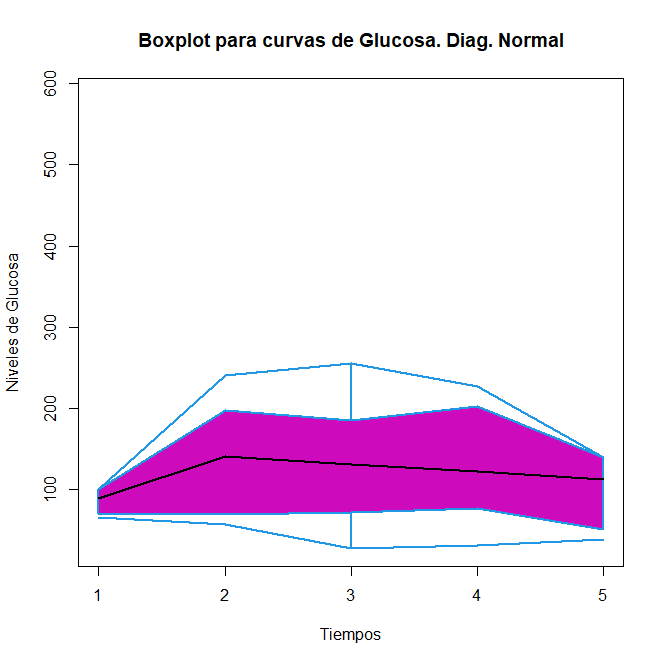
\includegraphics[width=0.45\textwidth]{img/bfgluNormal.png}}
  \subfloat[Insulina]{
   \label{bfInsNormal}
    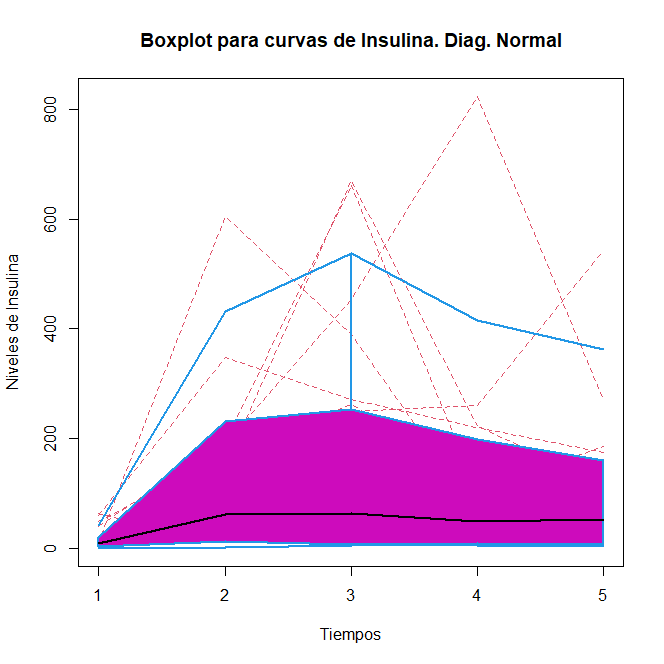
\includegraphics[width=0.45\textwidth]{img/bfInsNormal.png}}
    \caption{Boxplot funcional para las curvas de glucosa e insulina para personas con prediagnóstico normal.}
    \label{fig:bfNormal}
\end{figure}

La curva más profunda muestra un crecimiento muy suave desde el minuto 0 hasta el 30, para luego mantenerse con ligeras variaciones durante los próximos 90 minutos. Las curvas correspondientes al primer y tercer cuartil son muy distintas. El espacio entre la curva media y la del tercer cuartil es muy grande, indicando una gran variedad de rangos, aunque la forma se mantiene similar. Esto se puede interpretar como el inicio de una disminución en la eficiencia de la insulina sobre la glucosa. En cuanto a la curva del primer cuartil, tiene una forma y rango similar a la más profunda, lo que indica poca variabilidad en este conjunto. Aunque la forma de las curvas se mantiene consistente. Esto sugiere que, aunque hay diferencias en la cantidad de insulina producida, la respuesta general del cuerpo a la glucosa es bastante uniforme en este grupo.

\begin{figure}[H]
 \centering
  \subfloat[Glucosa]{
   \label{bfGluPre}
    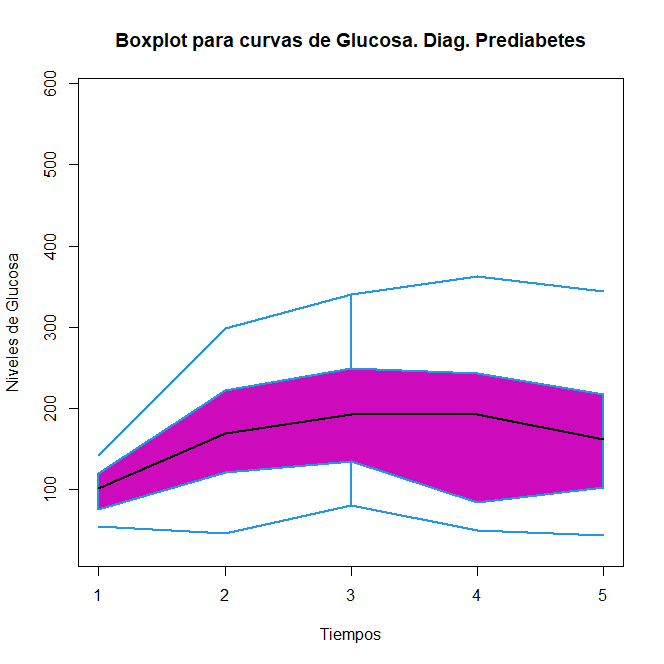
\includegraphics[width=0.48\textwidth]{img/bfgluPredia.png}}
  \subfloat[Insulina]{
   \label{bfInsPre}
    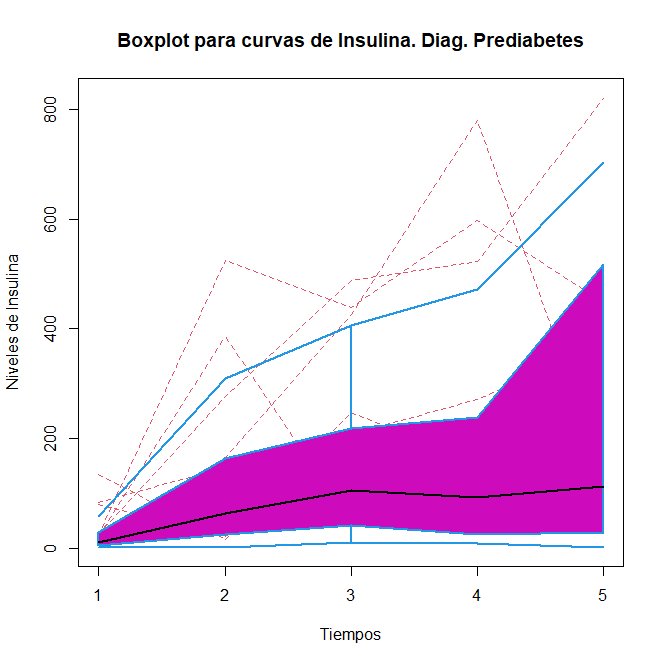
\includegraphics[width=0.48\textwidth]{img/bfInsPredia.png}}
    \caption{Boxplot funcional para las curvas de glucosa e insulina para personas con prediagnóstico prediabetes.}
    \label{fig:bfPrediabetes}
\end{figure}

La Figura \ref{bfGluPre} muestra el boxplot funcional de las curvas de glucosa para pacientes con prediagnóstico de prediabetes. Uno de los aspectos más destacables es el aumento en el rango de estas curvas en comparación con las de la categoría de diagnóstico normal. Por otra parte, la curva media aumenta suavemente hasta el minuto 90, para luego disminuir ligeramente en el minuto 120. Este comportamiento es similar para las curvas correspondientes al primer y tercer cuartil. Además, las distancias de estas curvas a la curva más profunda parecen ser similares, lo cual indica una varianza similar.

El boxplot de las curvas de insulina se puede ver en la Figura \ref{bfInsPre}. Se pueden apreciar datos atípicos, tanto en forma como en rango. Estos datos alcanzan niveles cercanos a 500 unidades, lo cual indica una sobreproducción de insulina y sugiere una posible falla de las células beta en un periodo de tiempo corto debido a nivel tan alto de hiperglucemia.

La curva más profunda muestra un crecimiento muy suave desde el minuto 0 hasta el 60, para luego mantenerse con ligeras variaciones durante los siguientes 60 minutos. Adicionalmente, las curvas correspondientes al primer y tercer cuartil son muy distintas. La curva del tercer cuartil es creciente en todo el dominio, lo cual indica una sobreproducción de insulina. Por otra parte, el espacio entre la curva media y la del tercer cuartil es muy grande, lo que indica una gran variedad en el rango y la forma de las curvas dentro de este subconjunto. Finalmente, la curva del primer cuartil parece tener una buena forma, ya que se encuentra muy pegada a la curva media. Así, el análisis del boxplot funcional de insulina revela una considerable variabilidad en la respuesta insulínica de los pacientes con prediagnóstico Prediabética. 


\begin{figure}[H]
 \centering
  \subfloat[Glucosa]{
   \label{bfGluDia}
    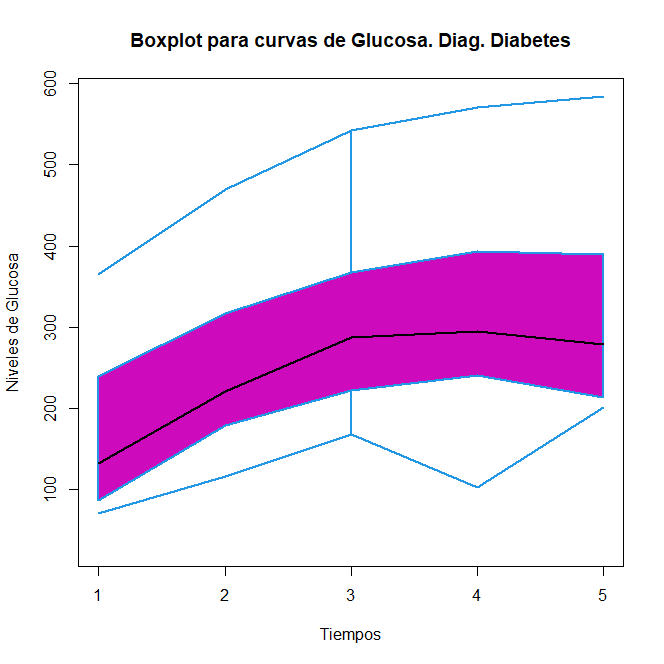
\includegraphics[width=0.48\textwidth]{Imagenes/fbGluDiabetes.png}}
  \subfloat[Insulina]{
   \label{bfInsDia}
    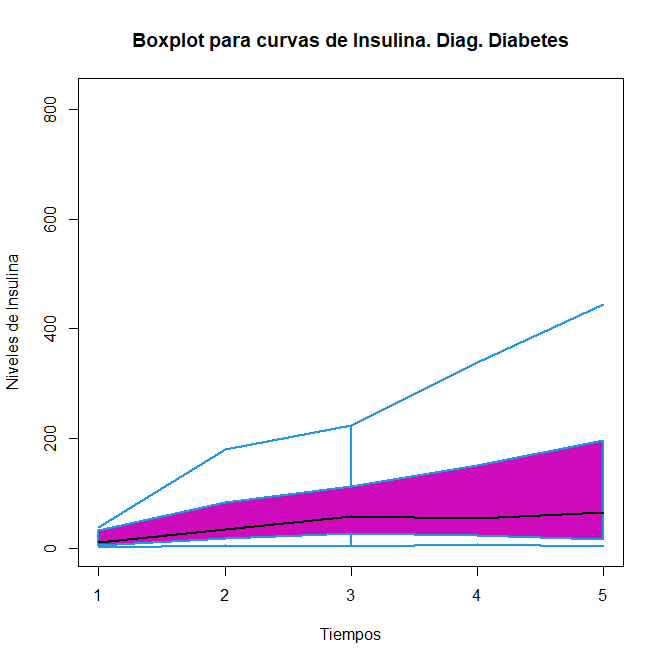
\includegraphics[width=0.48\textwidth]{img/bfInsDiabetes.png}}
    \caption{Boxplot funcional para las curvas de glucosa e insulina para personas con prediagnóstico diabético.}
    \label{fig:bfDiabetes}
\end{figure}

En la Figura \ref{bfGluDia}, se muestra el boxplot funcional de las curvas de glucosa de los pacientes con prediagnóstico de diabetes. Se observa que estas curvas abarcan un rango mucho mayor que las de las dos categorías anteriores, llegando incluso a valores cercanos a $600$. Además, la curva más profunda presenta un crecimiento más rápido que las otras dos y alcanza su punto máximo a los $90$ minutos, para luego disminuir ligeramente en los últimos $30$ minutos. Este comportamiento sugiere una respuesta casi nula de la insulina producida o de lo contrario la poca producción de insulina. 

Además, la separación entre las curvas relacionadas con el primer y tercer cuartil con respecto a la curva más profunda es mayor que en los casos anteriores, lo que indica una mayor varianza en los datos, aunque conservan la misma forma que la curva más profunda. Es importante destacar que en este gráfico no se muestran datos atípicos.

El boxplot funcional de las curvas para pacientes con prediagnóstico de diabetes se puede observar en la gráfica \ref{bfInsDia}. No se aprecia ningún valor atípico, sin embargo, la forma y el rango de estas curvas son muy diferentes a las curvas de insulina de los casos anteriores. Estas curvas presentan rangos muy bajos, lo que indica una disfunción en la producción de insulina por parte de las células beta. Además, las curvas muestran un comportamiento creciente durante todo el periodo de observación, lo que sugiere una mala respuesta de las células beta a la glucosa.  Este patrón se puede observar claramente en las curvas del primer y tercer cuartil, así como en la curva más profunda.

%%%%%%%%%%%%%%%%%%%%%%%%%%%%%%%%%%%%%%%%%%%%%%%%%%%%%%%%%%%%%%%%
%%%%%%%%%%%%%%%%%%%%%%%%%%%%%%%%%%%%%%%%%%%%%%%%%%%%%%%%%%%%%%%%

\subsection{Interacción de la Glucosa e Insulina}

Previamente se ha descrito cómo, de acuerdo con el avance de la enfermedad, la interacción entre la glucosa e insulina varía significativamente. En pacientes normales, se observaron curvas de insulina que aumentan y decrecen, manteniéndose en niveles bajos, mientras que las curvas de glucosa mostraban una mayor variabilidad. Por otro lado, en pacientes con prediagnóstico de prediabetes, la curva de insulina se encuentra en niveles más altos y, en algunos casos, no desciende, mientras que las curvas de glucosa son también más elevadas. Finalmente, en pacientes con diabetes, las curvas de insulina son variadas, pero en general no descienden, y las curvas de glucosa son consistentemente muy altas. El objetivo de esta subsección es clarificar la relación entre la glucosa e insulina que se quiere modelar.

\begin{figure}[H]
    \centering
    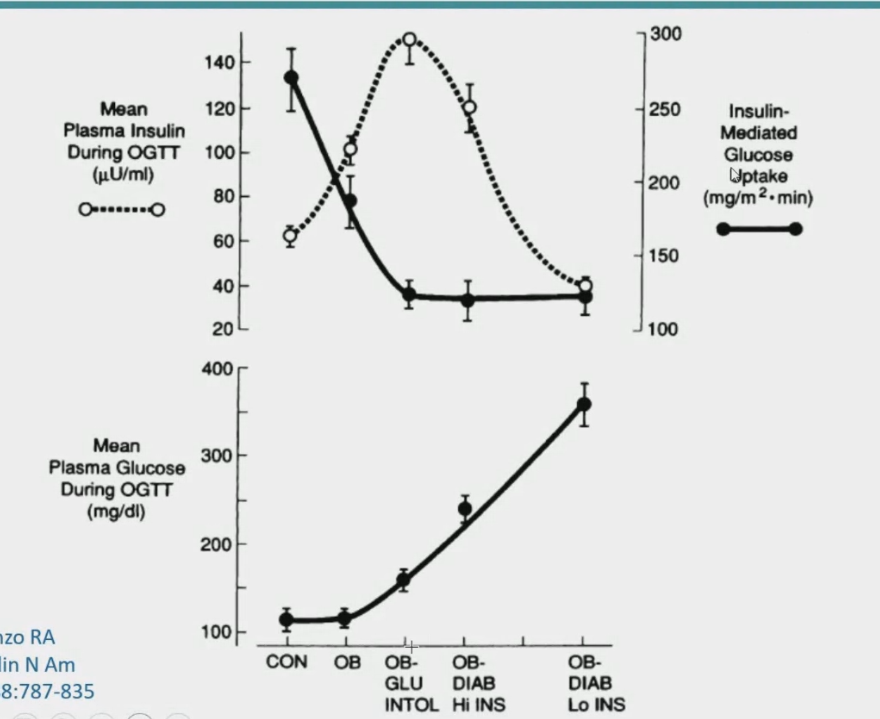
\includegraphics[width = 0.6 \textwidth]{Imagenes/InsulinaGlucosa.png}
    \caption{Relación de la glucosa e insulina por grado de enfermedad.}
    \label{fig:relGluIns}
\end{figure}

La Figura \ref{fig:relGluIns} fue tomada de una de las presentaciones de la Dra. Adriana Monroy. En ella se representan cinco grupos: el grupo control, personas con obesidad, personas con obesidad e intolerancia a la glucosa, personas con obesidad y diabetes con insulina alta, y personas con obesidad y diabetes con baja insulina. El objetivo es ilustrar cómo se comporta la interacción entre la glucosa e insulina dependiendo del estado de salud de los individuos.

En la gráfica de la parte inferior, se puede observar cómo, al empeorar la condición de salud, la media de los niveles de glucosa durante la prueba de tolerancia oral a la glucosa es más elevada. Este incremento en los niveles medios de glucosa refleja el deterioro progresivo en la regulación de la glucosa a medida que avanza la enfermedad.

Por otro lado, la gráfica de la parte superior muestra la captación de la glucosa medida por la insulina. En el grupo control, se observa que los niveles promedio de insulina en sangre son normales y la eficiencia de la insulina es buena. En el grupo de personas con obesidad, se puede ver cómo la producción de insulina es mayor, pero su eficiencia es menor, lo que indica posibles inicios de un trastorno metabólico.

A partir del grupo que presenta intolerancia a la glucosa, se puede observar cómo la eficiencia en la captación de glucosa llega a un límite. En las etapas siguientes, se evidencia el desgaste progresivo de las células beta del páncreas. En la última etapa, correspondiente a individuos con obesidad y diabetes con baja insulina, la producción de insulina es muy baja junto con su capacidad de absorción. Esto no solo refleja un deterioro avanzado en la regulación de la glucosa, sino también un agotamiento significativo de las células beta.

Estas observaciones subrayan la importancia de intervenir tempranamente en individuos con obesidad y aquellos que muestran signos de intolerancia a la glucosa. La progresión de la enfermedad desde la resistencia a la insulina hasta el agotamiento de las células beta resalta la necesidad de un monitoreo continuo y estrategias preventivas para evitar que la diabetes se vuelva irreversible.

%%%%%%%%%%%%%%%%%%%%%%%%%%%%%%%%%%%%%%%%%%%%%%%%%%
%%% A N A L I S I S  D E  R E S U L T A D O S %%%%
%%%%%%%%%%%%%%%%%%%%%%%%%%%%%%%%%%%%%%%%%%%%%%%%%%

\section{Interpretación de las Herramientas Visuales}

Dado el objetivo de crear un modelo simplificado, se va a construir un sistema que requiera un mínimo de variables, utilizando mediciones de fácil obtención. La variable de interés es $FBI/GC$, la cual se ha generado mediante el concepto de profundidad de banda con signo a partir de las curvas de glucosa e insulina, descrito en el Capítulo \ref{RegCuanDatosFun}. Las variables predictoras incluidas son los niveles de glucosa en ayunas y a los $120$ minutos durante la prueba de tolerancia a la glucosa oral, junto con el índice de masa corporal. Adicionalmente, se planea crear otro modelo al que se le añadirán mediciones de presión diastólica para explorar su efecto en la predicción de $FBI/GC$.

A continuación, se muestran las matrices de la $\sigma$ de Schweizer y Wolff, de hombres, mujeres y el total de la población, respectivamente. La correlación $\sigma$ de la variable respuesta el grupo de hombres es ligeramente mayor con todas las demás variables que en comparación con el caso de las mujeres.

\[
\sigma_{Muj} = \begin{blockarray}{cccccc}
FBI/GC      &      BMI      &    Glu.0      &  Glu.120      & PA.diast \\
\begin{block}{(ccccc)c}
1.000 & 0.311 & 0.542 &  0.733 & 0.181 & FBI/GC \\
0.311 & 1.000 & 0.304 &  0.308 & 0.261 & BMI \\
0.542 & 0.304 & 1.000 &  0.570 & 0.184 & Glu.0 \\
0.733 & 0.308 & 0.570 &  1.000 & 0.181 & Glu.120 \\
0.181 & 0.261 & 0.184 &  0.181 & 1.000 & PA.diast \\
\end{block}
\end{blockarray}
 \]

\[
\sigma_{Hom} = \begin{blockarray}{cccccc}
FBI/GC      &      BMI      &    Glu.0      &  Glu.120      & PA.diast \\
\begin{block}{(ccccc)c}
1.000 & 0.412 & 0.649 & 0.770 & 0.333 & FBI/GC \\
0.412 & 1.000 & 0.336 & 0.261 & 0.353 & BMI \\
0.649 & 0.336 & 1.000 & 0.591 & 0.312 & Glu.0 \\
0.770 & 0.261 & 0.591 & 1.000 & 0.282 & Glu.120\\
0.333 & 0.353 & 0.312 & 0.282 & 1.000 & PA.diast \\
\end{block}
\end{blockarray}
 \]


\[
\sigma_{Total} = \begin{blockarray}{cccccc}
FBI/GC      &      BMI      &    Glu.0      &  Glu.120      & PA.diast \\
\begin{block}{(ccccc)c}
1.000 & 0.361 & 0.567 & 0.747 & 0.244 & FBI/GC \\
0.361 & 1.000 & 0.324 & 0.320 & 0.317 & BMI \\
0.567 & 0.324 & 1.000 & 0.557 & 0.273 & Glu.0 \\
0.747 & 0.320 & 0.557 & 1.000 & 0.223 & Glu.120 \\
0.244 & 0.317 & 0.273 & 0.223 & 1.000 & PA.diast \\
\end{block}
\end{blockarray}
 \]

Todos los coeficientes resultantes de las matrices de correlación son lo suficientemente altos como para decir que hay algo que modelar con cópulas. De acuerdo con \cite{Erdely2022}, en este se enfatiza que si $\sigma_{C} = \rho_{C}$, entonces las variables aleatorias tienen una relación de dependencia de cuadrante positiva, y si $\sigma_{C} = -\rho_{C}$, entonces tienen una relación de dependencia de cuadrante negativa. Por otro lado, si $ |\rho_C| < \sigma_C$, significa que la dependencia es positiva en algunos cuadrantes y negativa en otros dentro del dominio de la cópula. Esto debido de a que $\rho_{C}$ es un valor promedio de dependencia del cuadrante, el cual podría ser cero.


La información anterior es beneficiosa durante el proceso de modelación, ya que una concordancia alta indica que el modelo paramétrico es capaz de capturar adecuadamente la estructura de dependencia entre las variables, mientras que una concordancia baja sugiere que el modelo podría no ser adecuado para describir la relación entre las variables. Además, es importante que el tipo de concordancia sea consistente en todo el dominio, ya que se requeriría de otras técnicas que pueden modelar este tipo de comportamiento, como el pegado de cópulas, entre otras.

A continuación, se muestran las matrices de diferencia:


\[
\sigma_{Muj} - \rho_{Muj} = \begin{blockarray}{cccccc}
FBI/GC      &      BMI      &    Glu.0      &  Glu.120      & PA.diast \\
\begin{block}{(ccccc)c}
  0.000 & 0.002 & -0.001 & -0.001  & -0.001 & FBI/GC \\
  0.002 & 0.000 &  0.002 &  0.004  & -0.001 & BMI \\
 -0.001 & 0.002 &  0.000 &  0.023  &  0.025 & Glu.0 \\
 -0.001 & 0.004 &  0.023 &  0.000  &  0.008 & Glu.120 \\
 -0.001 &-0.001 &  0.025 &  0.008  &  0.000 & PA.diast \\
\end{block}
\end{blockarray}
 \]

 \[
\sigma_{Hom} - \rho_{Hom} = \begin{blockarray}{cccccc}
FBI/GC      &      BMI      &    Glu.0      &  Glu.120      & PA.diast \\
\begin{block}{(ccccc)c}
0.000 & 0.004 & 0.002  & 0.000  & -0.003 & FBI/GC \\
0.004 & 0.000 & 0.007  & 0.013  &  0.002 & BMI \\
0.002 & 0.007 & 0.000  & 0.022  &  0.022 & Glu.0 \\
0.000 & 0.013 & 0.022  & 0.000  &  0.005 & Glu.120 \\
0.003 & 0.002 & 0.022  & 0.005  &  0.000 & PA.diast \\   
\end{block}
\end{blockarray}
 \]

 \[
\sigma_{Total} - \rho_{Total} = \begin{blockarray}{cccccc}
FBI/GC      &      BMI      &    Glu.0      &  Glu.120      & PA.diast \\
\begin{block}{(ccccc)c}
 0.000 & 0.002 & 0.002  & 0.000  &  0.008 & FBI/GC \\
 0.002 & 0.000 & 0.005  & 0.004  &  0.006 & BMI \\
 0.002 & 0.005 & 0.000  & 0.024  &  0.029 & Glu.0 \\
 0.000 & 0.004 & 0.024  & 0.000  &  0.016 & Glu.120 \\
 0.008 & 0.006 & 0.029  & 0.016  &  0.000 & PA,diast \\
\end{block}
\end{blockarray}
 \]

Las matrices de diferencias de los coeficientes $\rho$ de Spearman y $\sigma$ de Schweizer y Wolff presentadas anteriormente muestran valores muy bajos, lo cual indica que las dependencias entre las variables tienen un tipo de monotonía a lo largo de todo su dominio, es decir, son únicamente crecientes o decrecientes. Esta característica es beneficiosa al momento de ajustar cópulas, ya que sugiere que las cópulas paramétricas son una opción adecuada para modelar estas dependencias. Por esta razón, el modelo D-vine que se va a construir estará ajustado exclusivamente con cópulas paramétricas. Este enfoque permite capturar de manera efectiva las relaciones monotónicas entre las variables, mejorando la precisión y la interpretabilidad del modelo.



%%%%%%%%%%%%%%%%%%%%%%%%%%%%%%%%%%%%%%%%%%%%%%%%%%
%%%%%%%%%%%%%%%%%%%%%%%%%%%%%%%%%%%%%%%%%%%%%%%%%%

\subsection{Gráficos de dispersión y Heatmaps}

Para obtener una comprensión más profunda de cómo se ajusta cada cópula, se emplearon visualizaciones propuestas por Arturo Erdely y Manuel Rubio-Sanchez en \cite{Erdely2022}. Estas visualizaciones ofrecen una nueva perspectiva al representar la clásica gráfica de puntos de una manera innovadora, y al resaltar las diferencias entre la cópula empírica y la cópula independiente. Estas herramientas visuales ayudan a identificar patrones y estructuras de dependencia en los datos, lo que facilita la evaluación del ajuste de las cópulas y el análisis de la relación entre las variables. 

Recordando que las medidas $\rho_C$ y $\sigma_C$ se obtienen de medir la distancia entre la cópula empírica y la independiente, se proponen los heatmaps $\mathscr{H}_\rho$ y $\mathscr{H}_\sigma$ definidos en las ecuaciones \eqref{Hrho} y \eqref{Hsigma}, respectivamente, que visualizar esta distancia en distintos puntos del dominio de la cópula. Adicionalmente se propone el heatmap $\mathscr{H}$ definido en \eqref{H}, el cual muestra la distancia entre la cópula empírica y la independiente, con respecto a la cercanía con los limites de Frechet -Hoeffding:

\begin{equation}\label{Hrho}
    \mathscr{H}_\rho=\left\{12\left[C_n\left(\frac{i}{n}, \frac{j}{n}\right)-\frac{i j}{n^2}\right]: i, j \in\{1, \ldots, n-1\}\right\},
\end{equation}

\begin{equation}\label{Hsigma}
    \mathscr{H}_\sigma = \left\{12\left|C_n\left( \frac{i}{n}, \frac{j}{n}\right)-\frac{i j}{n^2}\right|: i, j \in\{1, \ldots, n-1\}\right\},
\end{equation}


\begin{equation}\label{D}
    D_n\left(\frac{i}{n}, \frac{j}{n}\right)=\left\{\begin{array}{cc}
\frac{C_n\left(\frac{i}{n}, \frac{j}{n}\right)-\Pi\left(\frac{i}{n}, \frac{j}{n}\right)}{M\left(\frac{i}{n}, \frac{j}{n}\right)-\Pi\left(\frac{i}{n}, \frac{j}{n}\right)} & \text { if } C_n\left(\frac{i}{n}, \frac{j}{n}\right) \geq \Pi\left(\frac{i}{n}, \frac{j}{n}\right), \\
-\frac{\Pi\left(\frac{i}{n}, \frac{j}{n}\right)-C_n\left(\frac{i}{n}, \frac{j}{n}\right)}{\Pi\left(\frac{i}{n}, \frac{j}{n}\right)-W\left(\frac{i}{n}, \frac{j}{n}\right)} & \text { if } C\left(\frac{i}{n}, \frac{j}{n}\right)<\Pi\left(\frac{i}{n}, \frac{j}{n}\right),
\end{array}\right. \quad \text{ para } i,j \in  \left\{ 1, \dots, n-1 \right\} 
\end{equation}

\begin{equation}\label{H}
    \mathscr{H} =\left\{ D_n\left( \frac{i}{n}, \frac{j}{n}\right) : i, j \in\{1, \ldots, n-1\}\right\}.
\end{equation}


Para iniciar con una visualización clásica, en la Figura \ref{fig:diagE} se muestran los gráficos de dispersión de las covariables dos a dos de los datos proveninetes de mujeres en escala $u$. En la diagonal superior se presentan las dispersión de las variables, mientras que en la diagonal inferior se muestran las diagonales de diferentes cópulas. La curva roja representa la diagonal de la cópula $W$, que corresponde a la cota inferior; en azul, se encuentra la diagonal de la cópula independiente; en verde la diagonal de la curva superior $M$, la cota superior; y por último, en negro se grafica la diagonal de la función empírica. Esta visualización ayuda a comprender las relaciones de concordancia presentes en cada variable, lo que facilita la elección de una estrategia adecuada al modelar con cópulas.

\begin{figure}[H]
    \centering
    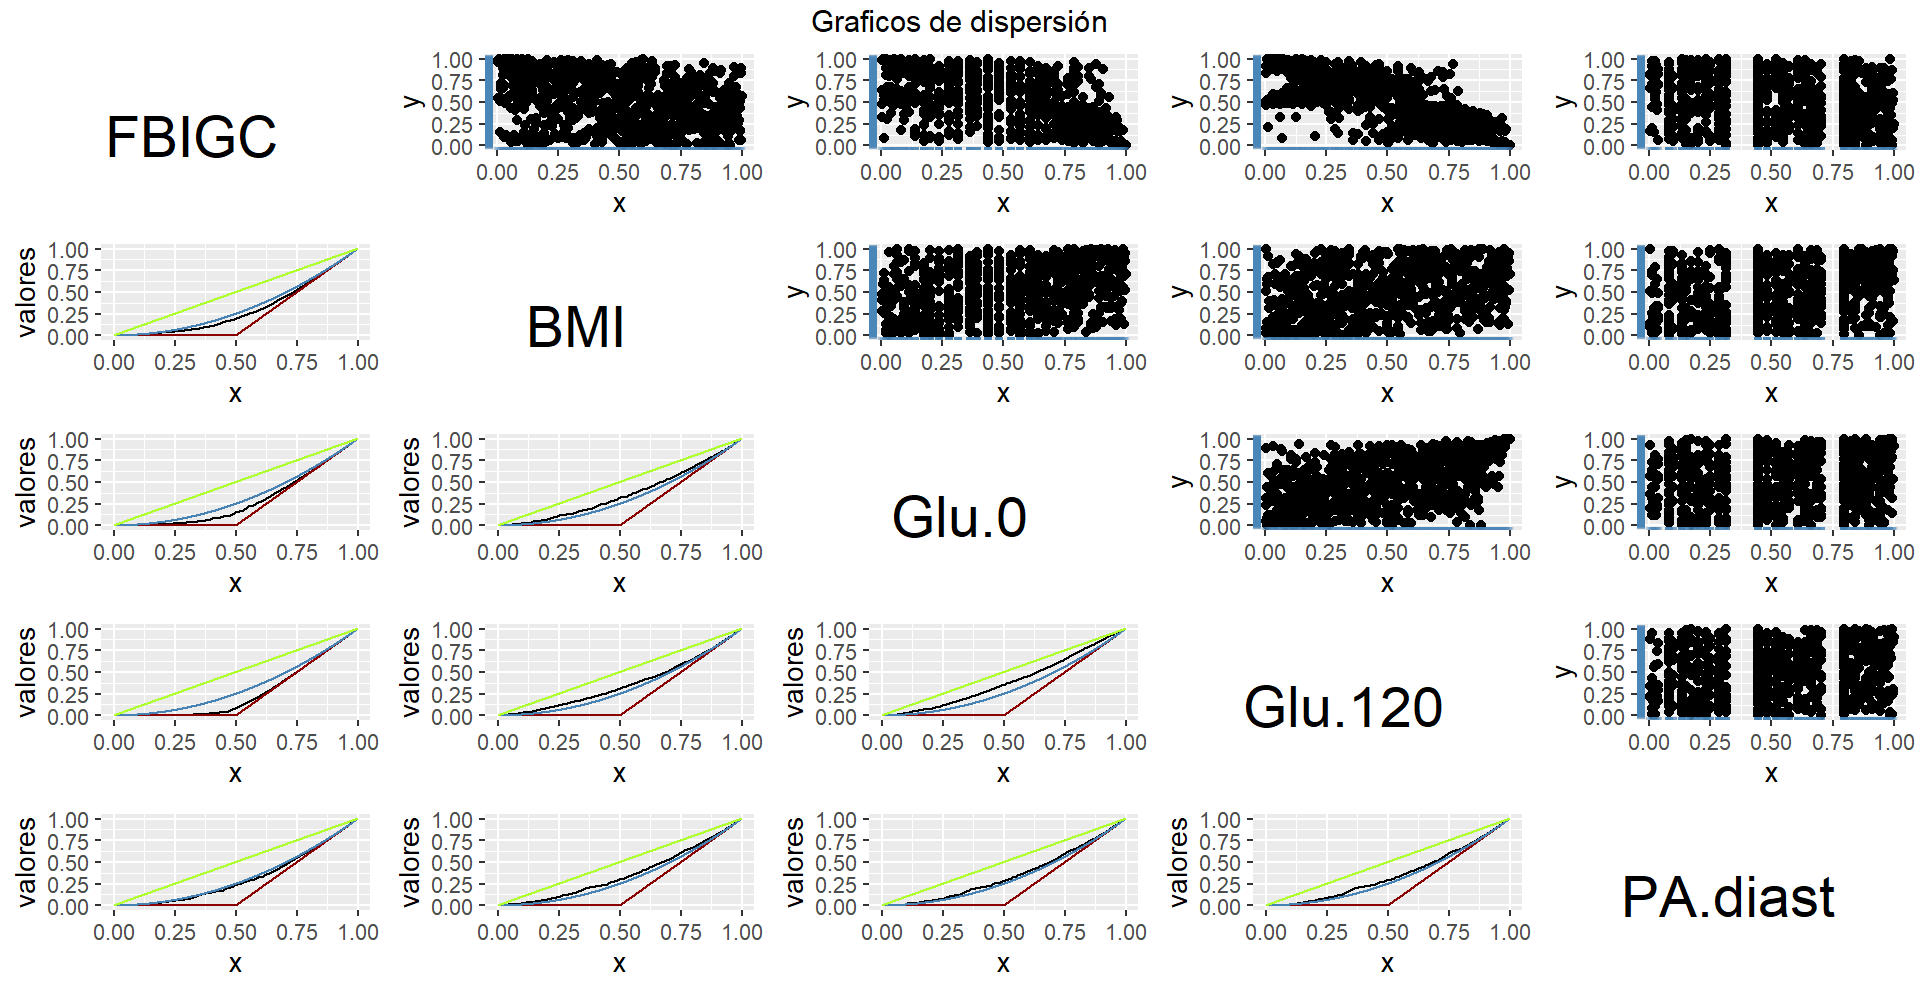
\includegraphics[width = 0.97 \textwidth]{4img/UdiagM.png}
    \caption{Diagonales y gráficos de dispersión en escala $u$.}
    \label{fig:diagE}
\end{figure}

Es importante tener en cuenta que aún falta explorar las dependencias entre las variables condicionales. Aunque los gráficos de dispersión proporcionan una visión general, también revelan ciertas franjas en los datos, lo cual puede indicar limitaciones potenciales del modelo (ver la diagonal superior de la Figura \ref{fig:diagE}). Esto se debe a que la mayoría de las cópulas paramétricas asumen datos continuos, y la presencia de franjas en los datos podría afectar la capacidad del modelo para capturar la verdadera estructura de dependencia entre las variables. Por lo tanto, es necesario realizar un análisis más detallado para comprender completamente la naturaleza de las dependencias y evaluar la idoneidad del modelo propuesto.

Ahora se aplicará los heatmaps anteriores a cópulas D-Vine. Para simplificar la notación del modelo D-vine, en lugar de escribir todos los árboles, solo se utilizará el árbol del primer nivel ya que este determina todas las estructuras subsecuentes, representándolo como un modelo aditivo. Esto se debe a su facilidad de comprensión y a la capacidad de trabajar con él en el entorno de fórmulas de \texttt{R}. Sin embargo, es importante tener en cuenta que esto no significa que en el modelado se asuma que las relaciones son aditivas. En realidad, se modelan las relaciones a pares de cópulas, lo que permite capturar una gama más amplia de estructuras de dependencia entre las variables.

En general, se asignará a cada variable que se modela un número, correspondiente al orden en el que el modelo D-vine las ajusta. Por ejemplo, en el modelo $FBI/GC \sim GLU.120 + GLU.0 + IBM + PA.diast$, la variable $1$ corresponderá a la variable respuesta $FBI/GC$, la variable $2$ a $Glu.120$, y así sucesivamente. Cuando se modele la dependencia entre dos variables utilizando cópulas, se utilizará el número de variable como subíndice. Por ejemplo, $C_{12}$ representaría la cópula entre $FBI/GC$ y $Glu.120$.


\begin{figure}[H]
 \centering
  \subfloat[$\mathscr{H}\rho$]{
   \label{rhoT}
    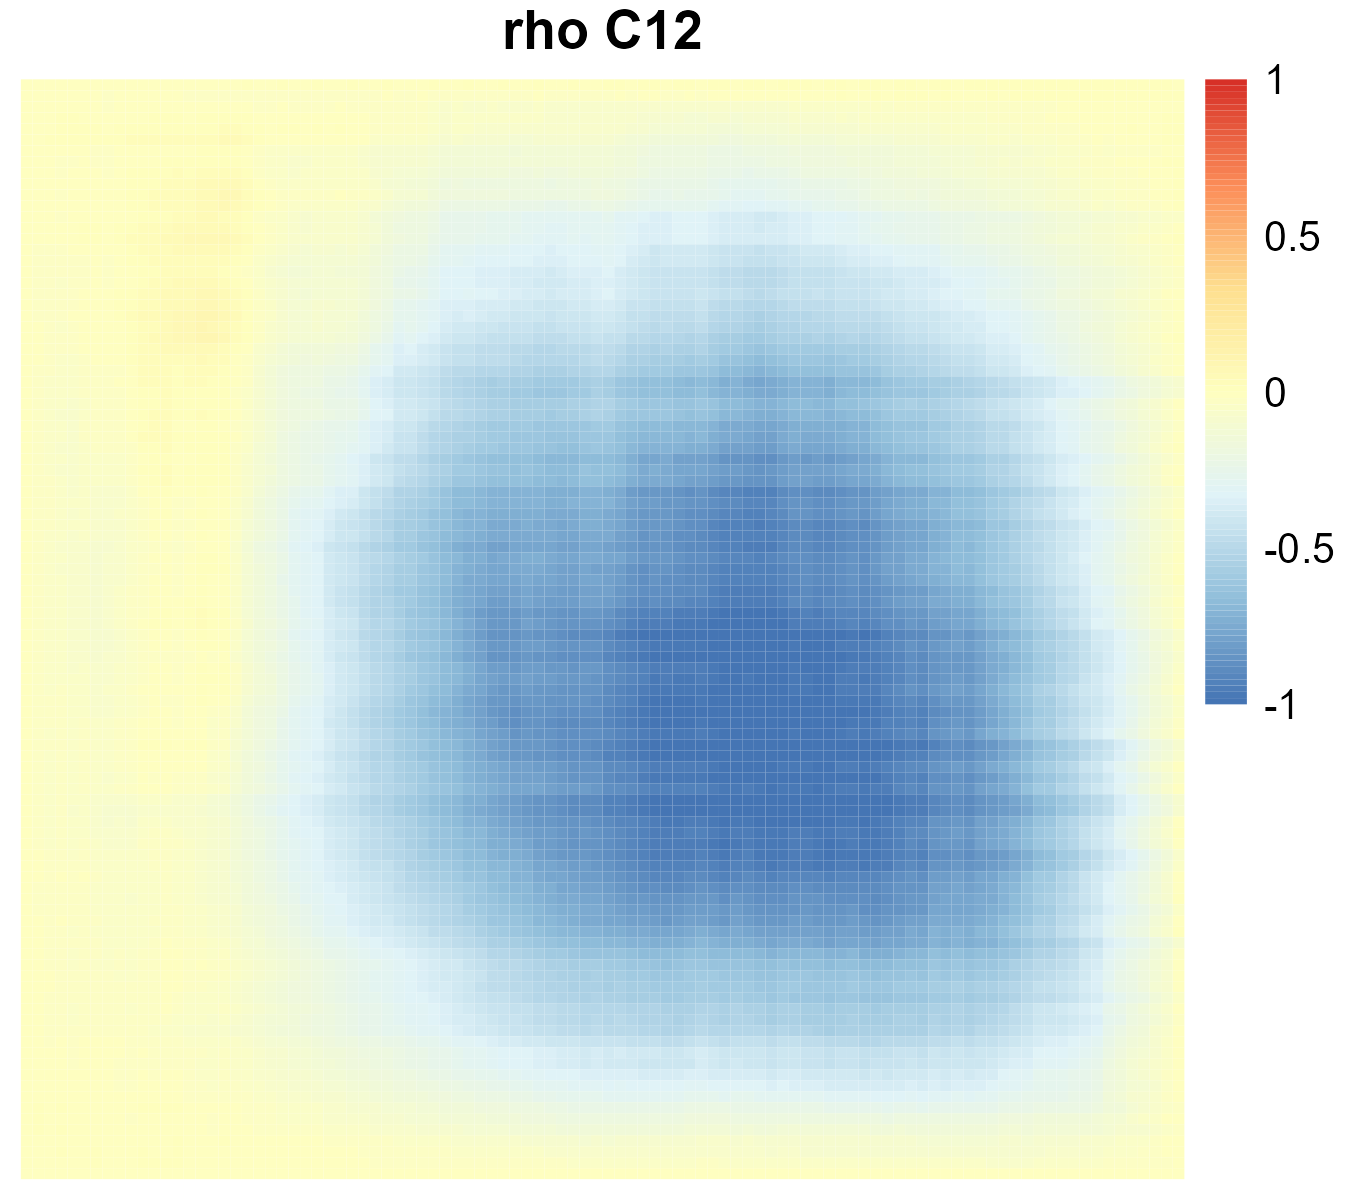
\includegraphics[width=0.32\textwidth]{4img/TotalrhoC12.png}}
  \subfloat[$\mathscr{H}\sigma$]{
   \label{sigmaT}
    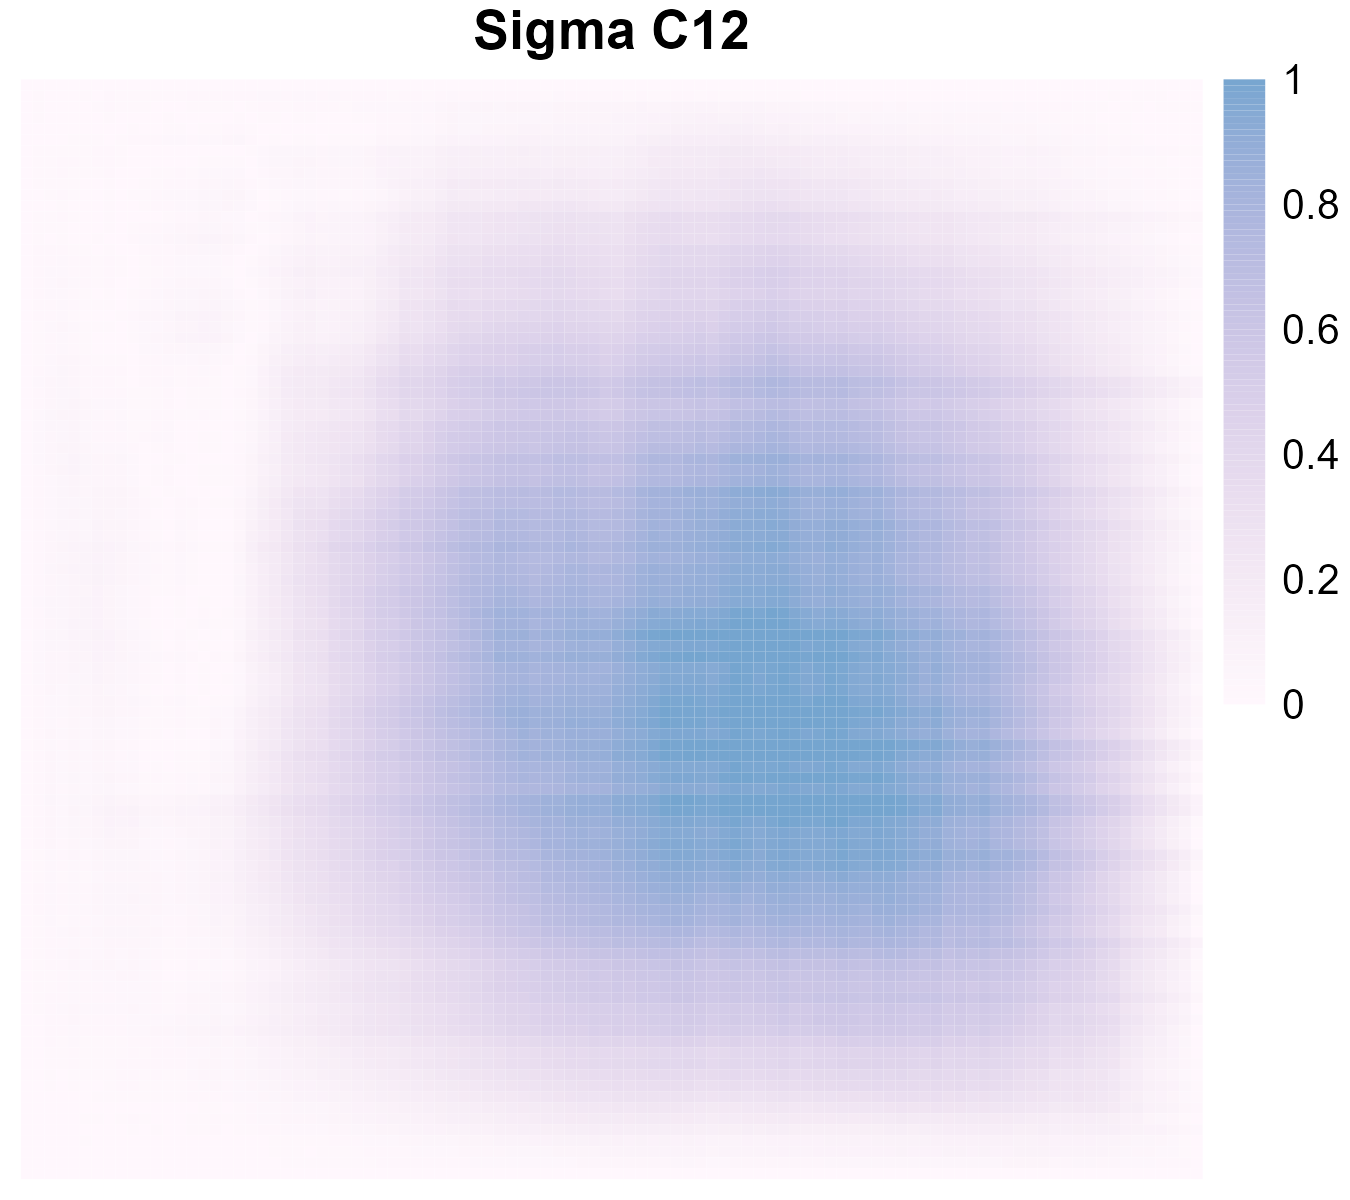
\includegraphics[width=0.32\textwidth]{4img/TotalsigmaC12.png}}
  \subfloat[$\mathscr{H}$]{
   \label{HT}
    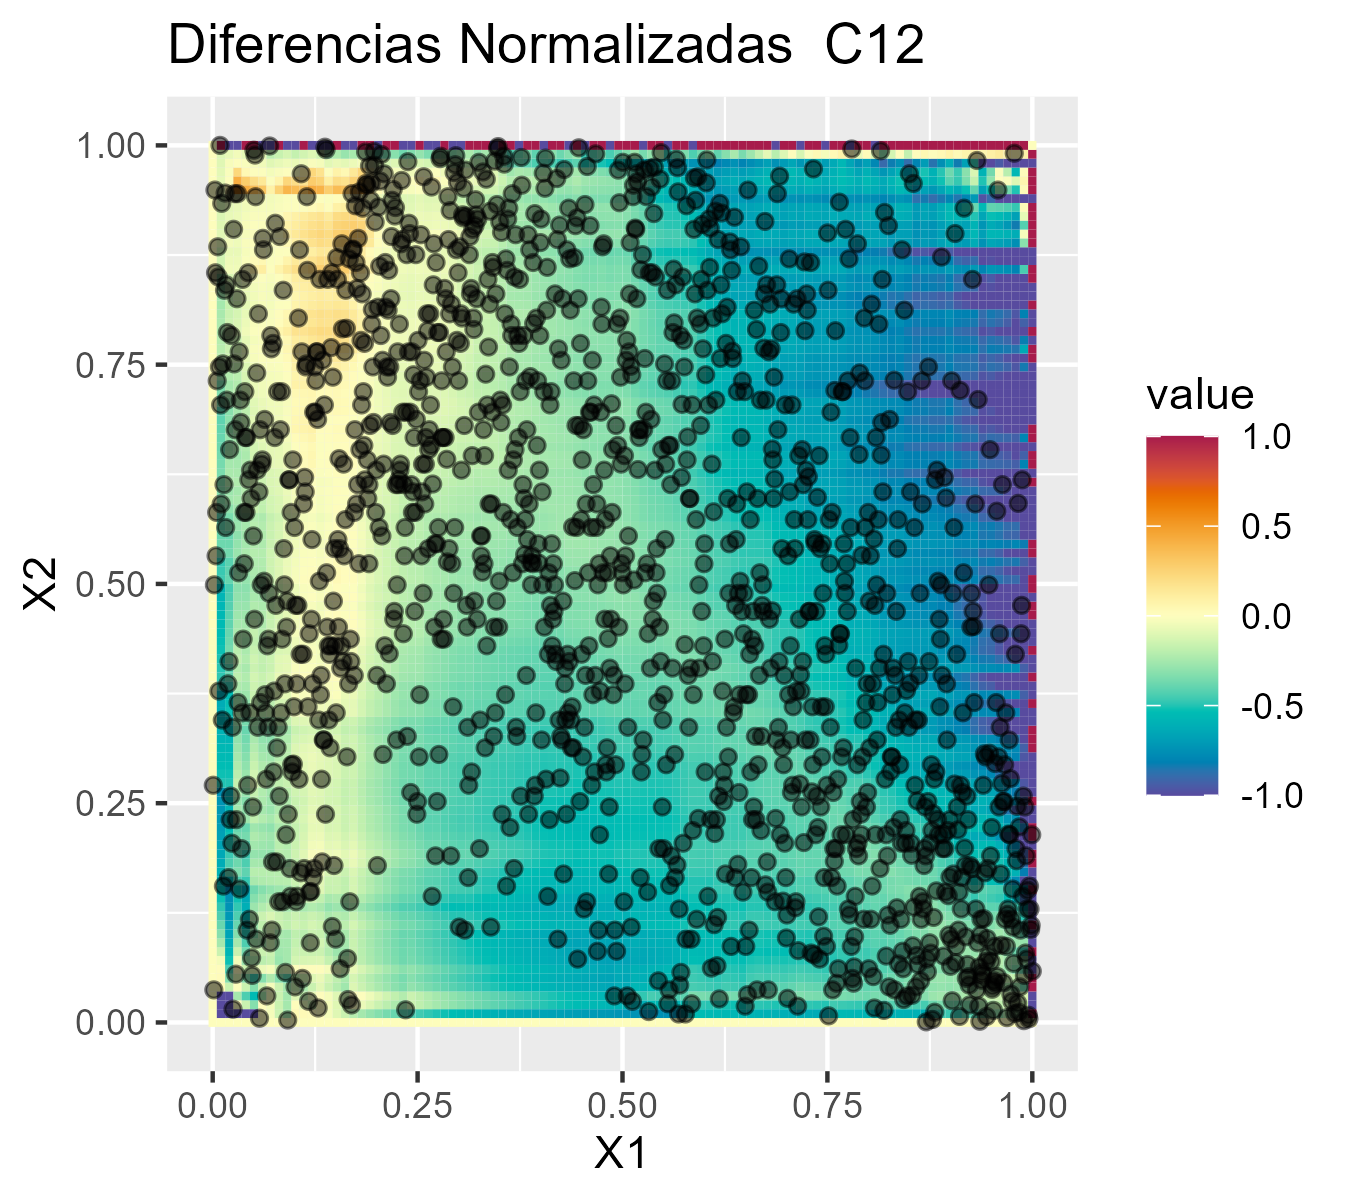
\includegraphics[width=0.32\textwidth]{4img/TotalHC12.png}}
    \caption{Ejemplo de Heatmaps}
    \label{heatEj}
\end{figure}

La Figura \ref{heatEj} presenta los heatmaps \eqref{Hrho}, \eqref{Hsigma} y \eqref{H} aplicados a la cópula entre $FBI/GC$ y $Glu.120$ para la cópula D-vine discutida arriba; más detalles sobre el ajuste de este modelo se presentan abajo. Como guía para interpretar los heatmaps, en la primera columna de la Figura \ref{heatEj}, se muestra la medida $\rho_C$ de Spearman en una cuadrícula de $100$ por $100$ en el intervalo $[0, 1]^2$. Las áreas azules indican que la distancia entre la cópula empírica evaluada en el punto $(u, v)$ está por debajo de la cópula independiente. Por otro lado, si los valores son positivos, esto indicará que la cópula empírica está por encima de la cópula independiente y su color será rojo. Este gráfico ayuda a visualizar el comportamiento de la cópula en todo el dominio, proporcionando información sobre la dirección y la magnitud de las diferencias entre la cópula empírica y la independiente.

En la segunda columna de la Figura \ref{heatEj}, se encuentra el heatmap con la medida $\sigma_C$. Esta medida solo evalúa la distancia entre la cópula empírica y la independiente sin considerar su signo. Esto nos ayuda a visualizar la magnitud de la dependencia en todo el dominio de la cópula, proporcionando una representación clara de la fuerza de la relación entre las variables.

Finalmente, el heatmap de la tercera columna de la Figura \ref{heatEj}, muestra las diferencias con normalización. Esto permite observar la presencia de tendencias crecientes y decrecientes en la relación entre las variables. Además, se sobreponen los datos con los que se estimó la cópula para ofrecer mayor claridad en la interpretación de los datos, lo que facilita la identificación de patrones y estructuras de dependencia en el conjunto de datos analizado.

%%%%%%%%%%%%%%%%%%%%%%%%%%%%%%%%%%%%%%%%%%%%%%%%%%%%%%%%%%%%%
%%%%%%%%%%%%%%%%%%%%%%%%%%%%%%%%%%%%%%%%%%%%%%%%%%%%%%%%%%%%%

\subsection{Tabla Resumen de Pertenencia a cada Clase}\label{subTabla}

Para generalizar el modelo, se separan a los individuos según su prediagnóstico, que proviene de la información de glucosa en los tiempos $0$ y $120$, así como su clasificación de nivel de obesidad según el Índice de Masa Corporal. A continuación se mencionan estas categorías propuesta por el Dr. Arnulfo González Cantú:

\begin{multicols}{2}
    \begin{itemize}
        \item Normal-Peso Normal
        \item Normal-Sobrepeso
        \item Normal-Obesidad	
        \item Prediabetes-Peso Normal
        \item Prediabetes-Sobrepeso
        \item Prediabetes-Obesidad	
        \item Diabetes-Peso Normal	
        \item Diabetes-Sobrepeso
        \item Diabetes-Obesidad
    \end{itemize}
\end{multicols}

Al categorizar a los individuos de esta manera, se puede analizar la relación entre las variables en diferentes subgrupos, lo que puede ayudar a identificar patrones específicos y a adaptar el modelo a las necesidades particulares de cada grupo.

Dividiendo a los individuos en las clasificaciones mencionadas anteriormente, se puede obtener la mediana de cada covariable para cada grupo y luego ingresar estas medianas al modelo para calcular la probabilidad de pertenecer a cada clase del $FBI/GC$, que incluyen las siguientes categorías: completamente sanos, resistencia a la insulina con predisfunción de célula beta, resistencia a la insulina con estrés de célula beta y resistencia a la insulina con disfunción obvia de célula beta. Este enfoque nos permite evaluar cómo varían las probabilidades de pertenecer a cada clase según las características de los individuos, lo que puede proporcionar información valiosa para la detección temprana y la intervención en diferentes estados de salud relacionados con la glucosa y la obesidad.

La tabla resultante del trabajo descrito anteriormente es fácilmente manejable y se puede utilizar de la siguiente manera:

\begin{enumerate}
    \item Ubicar la fila que corresponde a cada individuo colocando las medidas de glucosa en el tiempo $0$ ($Glu.0$), en el tiempo $120$ ($Glu.120$) y el Índice de Masa Corporal ($BMI$), de acuerdo a las clasificaciones descritas \ref{ClasificaVar}.

    \item En las columnas $C_1$, $C_2$, $C_3$, $C_4$, se muestran las probabilidades correspondientes a cada clase del $FBI/GC$ (completamente sanos, resistencia a la insulina con predisfunción de célula beta, resistencia a la insulina con estrés de célula beta y resistencia a la insulina con completa disfunción de célula beta, respectivamente).
\end{enumerate}

En la Figura \ref{fig:ejemploTabla}, se muestra un ejemplo. Esta tabla facilita la evaluación de las probabilidades de pertenecer a cada clase del $FBI/GC$ para diferentes combinaciones de glucosa y $BMI$, lo que permite una rápida identificación de los grupos de riesgo y la toma de decisiones informadas sobre la salud y el tratamiento. Estas predicciones de cada grupo de pacientes se obtuvieron tomando la mediana de cada covariable por cada grupo.

\begin{figure}[H]
    \centering
    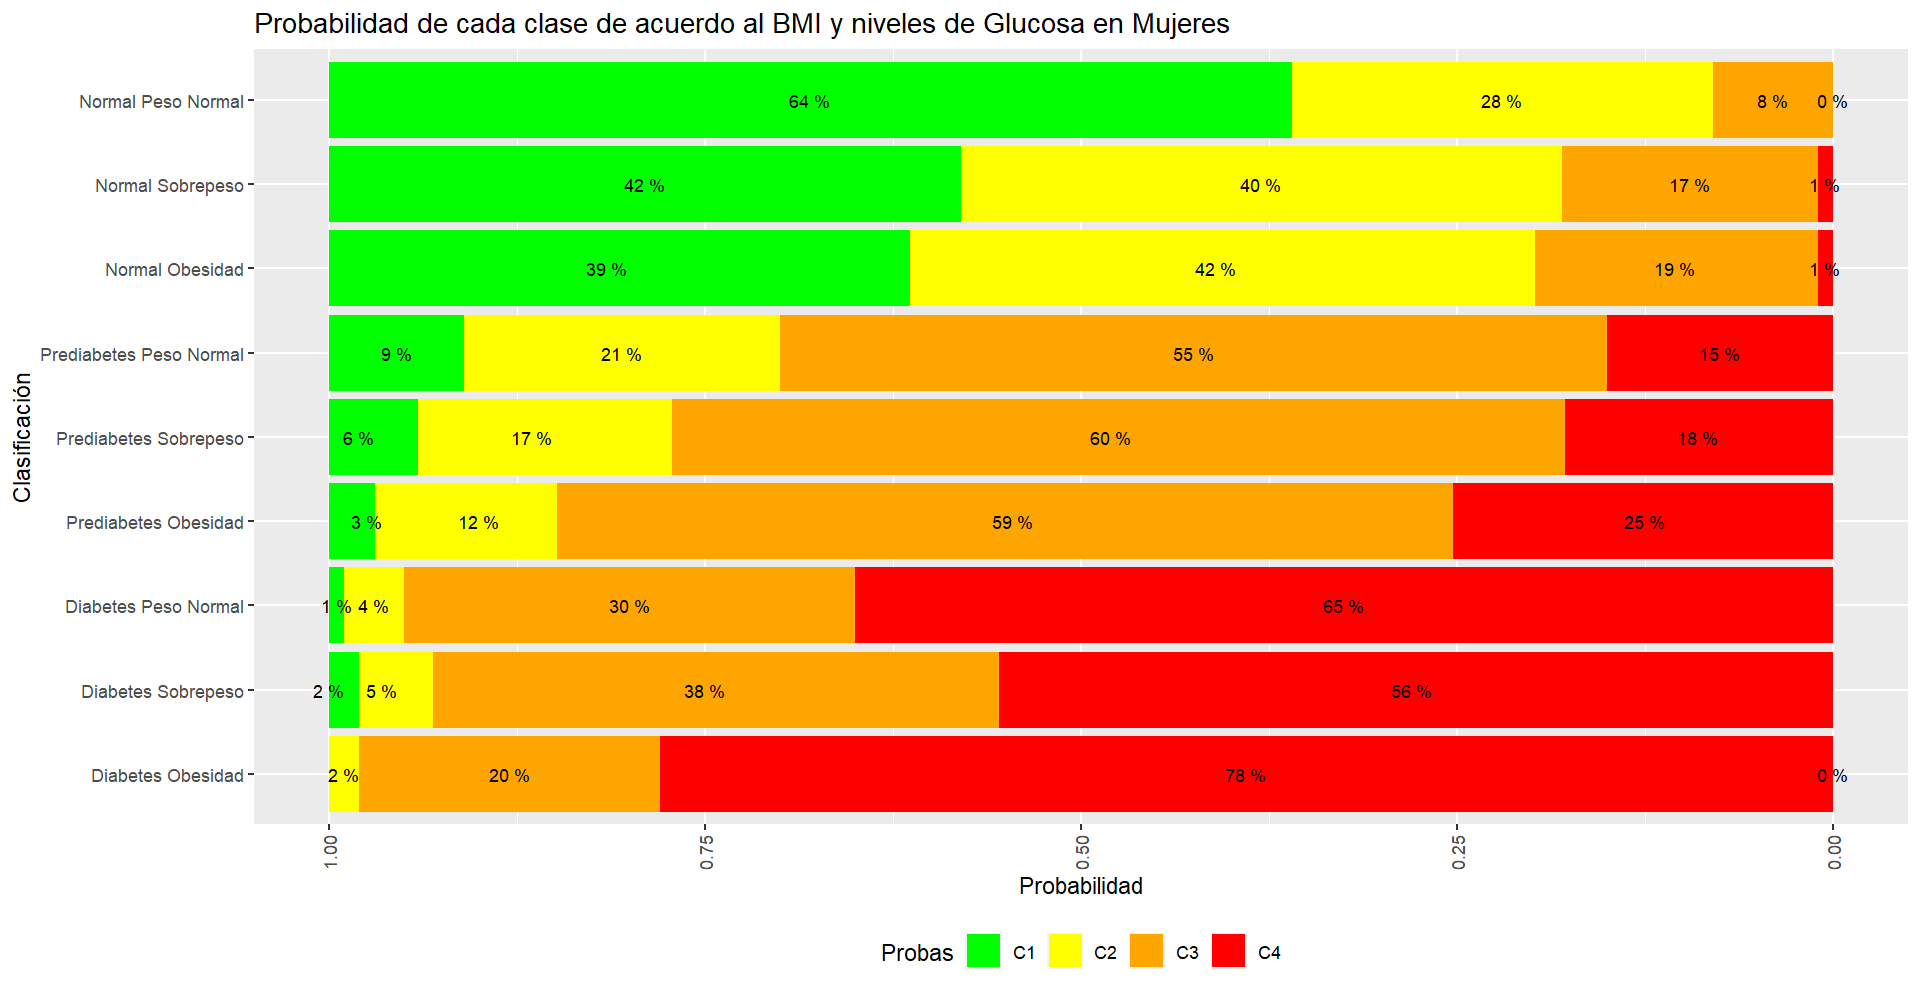
\includegraphics[height = 12 cm, width = 0.98 \textwidth]{4img/tablaM.png}
    \caption{Tabla de probabilidades de cada clase.}
    \label{fig:ejemploTabla}
\end{figure}

Para el cálculo de las probabilidades en esta tabla, solo se calcularon las siguientes probabilidades:

\begin{equation}
     \begin{matrix}
\mathbb{P}[0 \leq Y \leq 1] = C_1 \\
\mathbb{P}[-1 \leq Y \leq 0] = C_2  \\
\mathbb{P}[-2 \leq Y \leq -1] = C_3 \\
\mathbb{P}[-3 \leq Y \leq -2] = C_4 \\
\end{matrix}
\end{equation}
%%%%%%%%%%%%%%%%%%%%%%%%%%%%%%%%%%%%%%%%%%%%%%%%%%%%%%
%%%%%%%%  g r a f i c a   d e  e f e c t o s %%%%%%%%%
%%%%%%%%%%%%%%%%%%%%%%%%%%%%%%%%%%%%%%%%%%%%%%%%%%%%%%

\subsection{Gráfica de Efectos}

Las gráficas de efectos ofrecen una herramienta valiosa para visualizar el impacto marginal de un predictor en el estimador cuantil. Estas representaciones permiten observar cómo varía el estimador cuantil en respuesta a cambios en un predictor específico, mientras se mantienen los demás predictores constantes a su valor promedio \cite{Tepegjozova2022}.

Para generar estas gráficas, se selecciona la variable $x_i$ de interés cuyo efecto se desea visualizar en la regresión. Luego, se calcula el promedio muestral de todas las otras variables como una estimación de la esperanza de cada una. De esta manera, solo es de interés el comportamiento de la variable respuesta $y$ cuando la variable $x_i$ varia, mientras que todas las demás variables se mantienen constantes en su valor promedio. Posteriormente, se realiza la regresión cuantil utilizando estos valores fijos para las variables control.

A continuación, se presenta un ejemplo del rendimiento de la gráfica de efectos. Se llevó a cabo la regresión cuantil para tres cuantiles diferentes: $\alpha = 0.1$, $0.5$ y $0.9$. Luego, se utilizó la función $geom\_smooth()$ para trazar una curva suave utilizando B-splines con 5 puntos internos. 

\begin{figure}[H]
 \centering
  \subfloat[Mujeres]{
   \label{ejEfec1}
    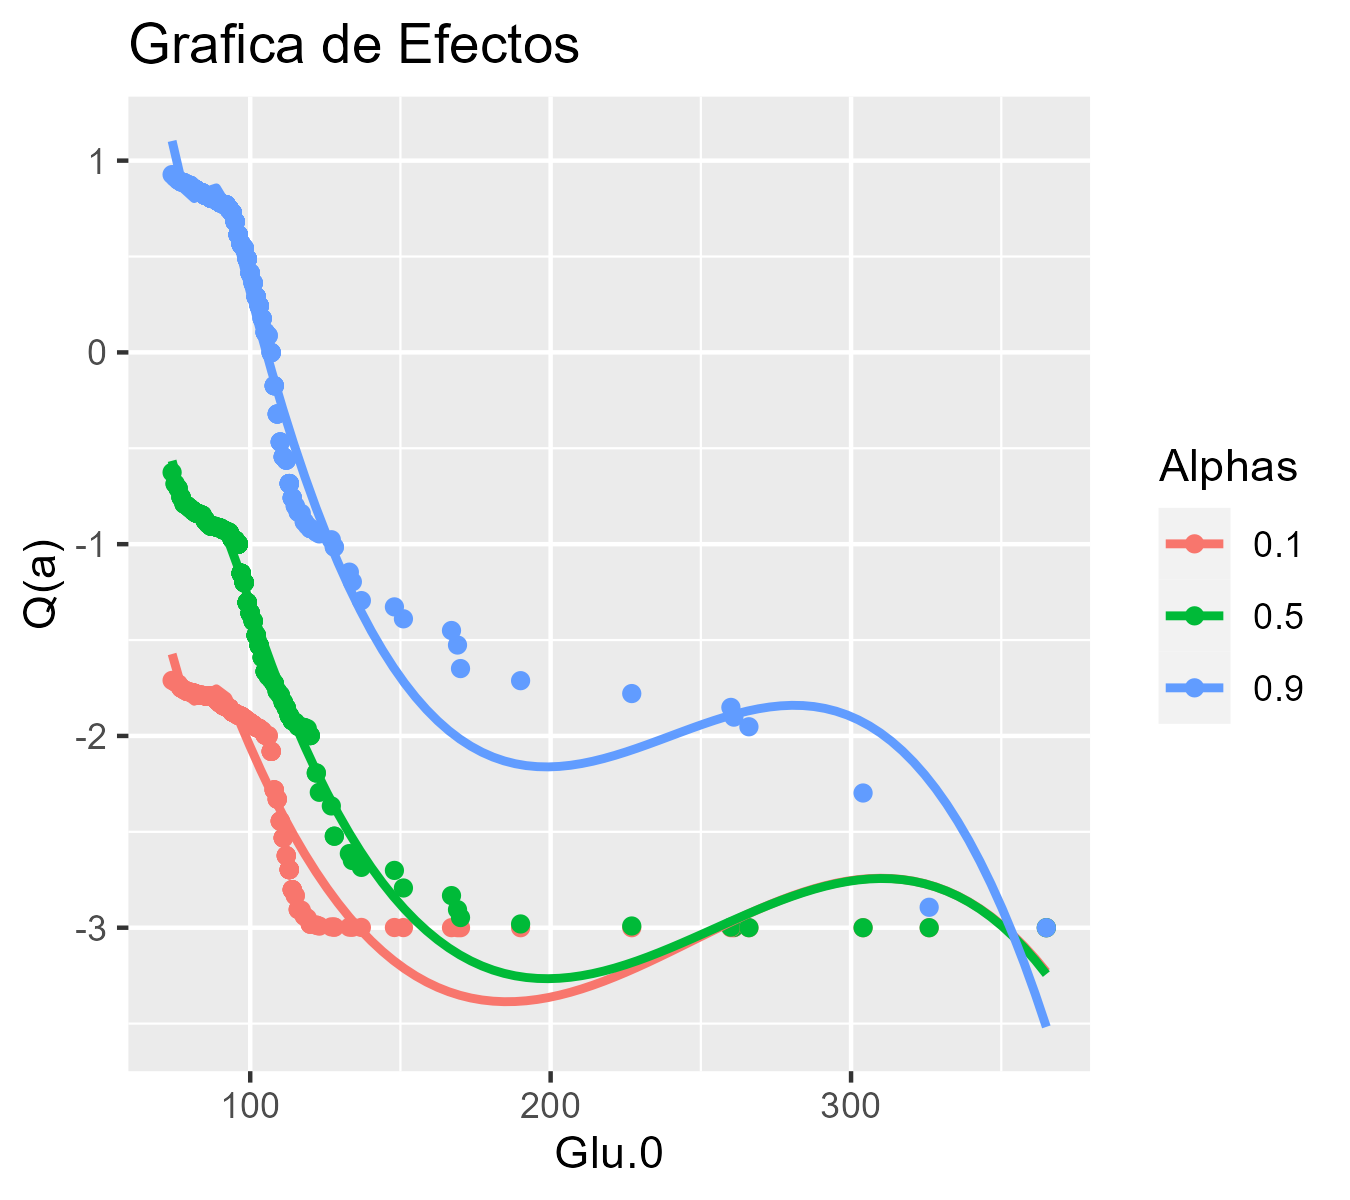
\includegraphics[width=0.45\textwidth]{4img/HomGlu.0Efec.png}}
  \subfloat[Hombres]{
   \label{ejEfect2}
    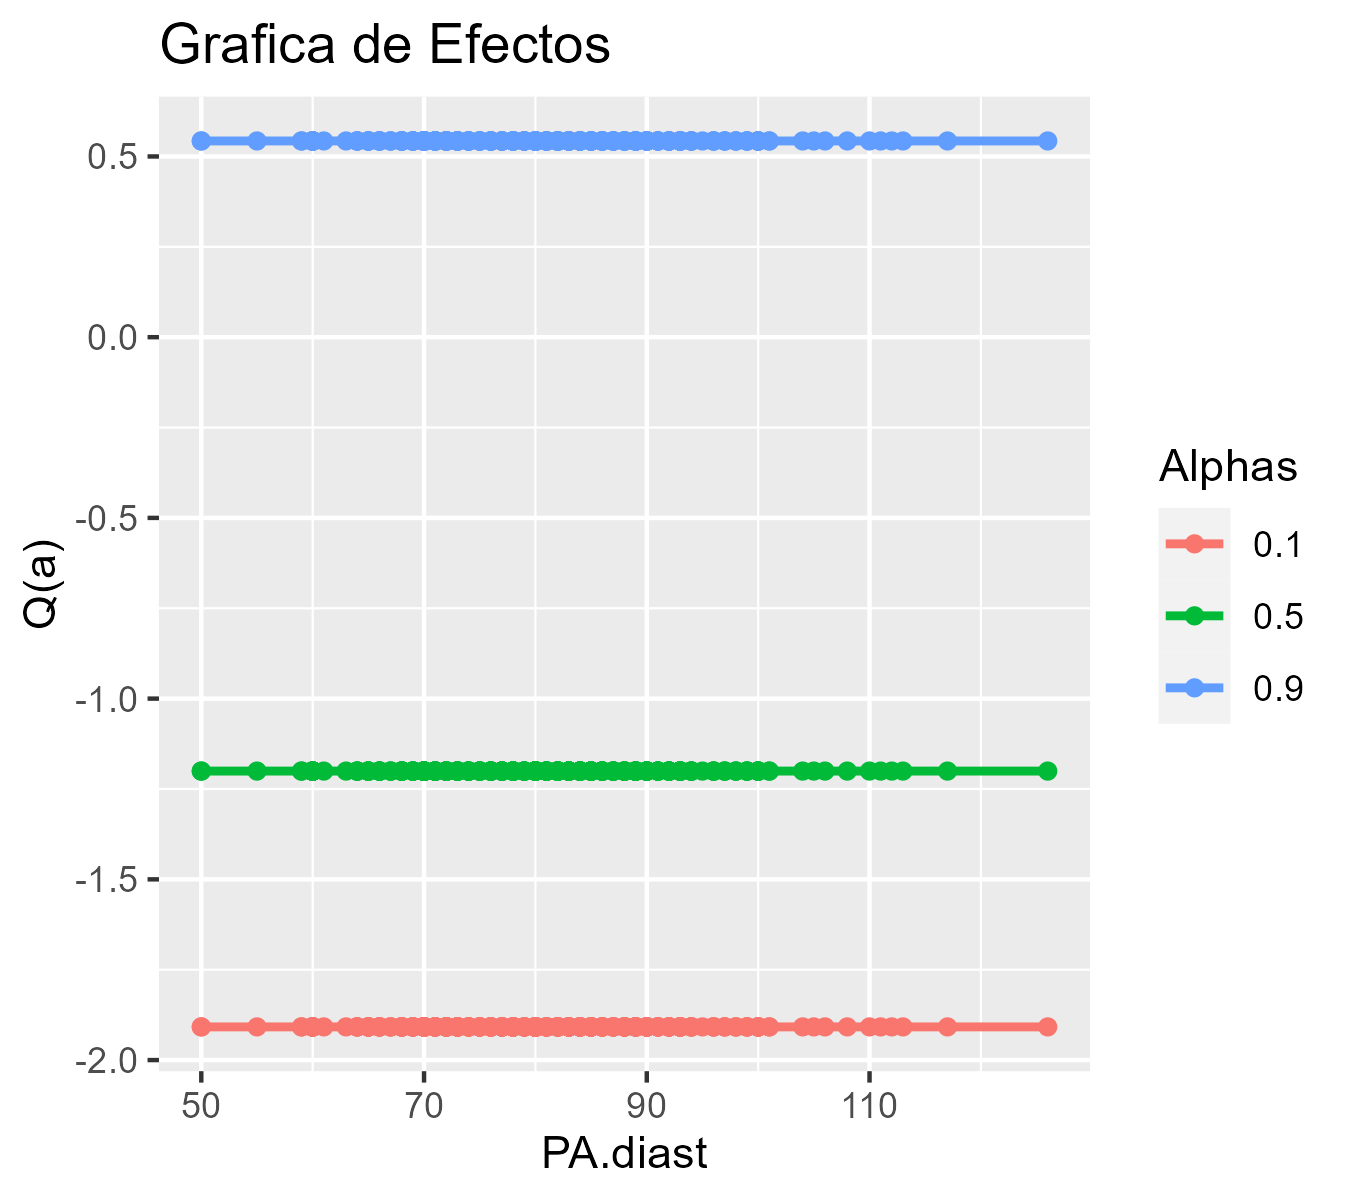
\includegraphics[width=0.45\textwidth]{4img/HomPA.diastEfec.png}}
    \caption{Ejemplos de las gráficas de efectos.}
    \label{fig:Efectos}
\end{figure}

En la Figura \ref{ejEfec1}, se ilustra cómo cambia la variable respuesta en función de los distintos valores de la variable $Glu.0$. Esto se puede entender como un boxplot continuo y puede ayudar a visualizar cómo varía la respuesta entre diferentes configuraciones del sistema. Al observar los boxplots, se puede identificar rápidamente qué configuraciones resultan en respuestas más consistentes (menor variabilidad) y cuáles tienen tiempos de respuesta más rápidos (mediana más baja). Por ejemplo, al final de esta gráfica, los datos también representan casos atípicos para la covariable que se está variando. Sin embargo, la respuesta deja de variar en estos casos debido a la menor cantidad de datos y la condición médica específica. Esta disminución en la variabilidad puede indicar que, en estas condiciones extremas, la respuesta se vuelve más uniforme, posiblemente debido a limitaciones fisiológicas.


Por otro lado, en la Figura \ref{ejEfect2}, se muestra el efecto de una variable que no aporta información al modelo. A medida que la covariable $PA.diast$ varía, no se refleja ningún cambio en la predicción; esto permanece constante. Esto indica que  $pA.diast$ no aporta información significativa a la regresión. La ausencia de variación en la respuesta sugiere que esta covariable no está relacionada con la variable de interés y, por lo tanto, no contribuye a mejorar el modelo predictivo. Identificar tales variables es crucial para simplificar el modelo y mejorar su interpretabilidad y eficiencia.


Este gráfico es herramienta fundamental en el análisis de resultados debido a su capacidad para visualizar de manera efectiva la variabilidad y la relación entre una covariable y la variable respuesta. En particular, permiten identificar patrones claros en los datos, como la consistencia en la respuesta frente a diferentes condiciones de una covariable o la falta de efecto de ciertas variables sobre la predicción. Esta capacidad de identificación es crucial para la selección de variables relevantes en los modelos predictivos y para mejorar la interpretación y la precisión de los resultados obtenidos. 

%%%%%%%%%%%%%%%%%%%%%%%%%%%%%%%%%%%%%%%%%%%%%%%%%%%%%%%%%%%%%%%%
%%%%%%%%%%%%%%%%%%%%%%%%%%%%%%%%%%%%%%%%%%%%%%%%%%%%%%%%%%%%%%%%

\vspace{-0.2cm}
\section{Librería deerVineReg}

\vspace{-0.3cm}
Todas las herramientas gráficas descritas anteriormente para evaluar y visualizar el desempeño del modelo ajustado fueron implementadas en el paquetería \textbf{deerVineReg}, la cuál se puede encontrar y descargar en github \url{https://github.com/BesitosDeBaba/deerVineReg}, uno de los principales objetivos de esta tesis. Existen otros paquetes, como \textbf{vineReg}, cuya utilidad se centra más en visualizar las dependencias dentro de un conjunto de variables, similar a la función de la PCA. Sin embargo, este proyecto se enfocó en desarrollar una paquetería orientada a un modelo predictivo de Machine Learning, con el objetivo de expandir el uso de modelos basados en cópulas.

El paquete \textbf{deerVineReg} no solo facilita la creación de modelos predictivos robustos utilizando cópulas, sino que también incluye herramientas avanzadas de visualización para interpretar los resultados y evaluar el desempeño del modelo. Esto permite a los usuarios no solo construir modelos precisos, sino también comprender mejor las relaciones subyacentes entre las variables y su impacto en la predicción. \textbf{deerVineReg} representa un avance significativo en el uso de cópulas para la predicción, ofreciendo una alternativa poderosa y accesible para la comunidad científica y médica.

%%%%%%%%%%%%%%%%%%%%%%%%%%%%%%%%%%%%%%%%%%%%%%%%%%%%%%%%%%%%%
%%%%%%%%%%%%%%%%%%%%%%%%%%%%%%%%%%%%%%%%%%%%%%%%%%%%%%%%%%%%%
\section{Modelos de 4 variables}

El orden de los tres modelos modelos construidos para el diagnóstico de la resistencia a la insulina en mujeres, hombres y para ambos sexos es

\vspace{-0.5cm}
\begin{equation}\label{ordenVar4}
     FBI/GC \sim Glu.120 + Glu.0 + BMI + PA.diast.
\end{equation}

Las cópulas ajustadas para los datos de mujeres se ilustran en la Figura \ref{fig:copulasTestMu}, mientras que las correspondientes a hombres se muestran en la Figura \ref{fig:copulasTestHo}.


Para ajustar las cópulas a pares de todos los niveles, se utilizó la función \textit{BiCopSelect} de la librería \textbf{VineCopula}. En las Figuras  \ref{fig:copulasTestMu}, \ref{fig:copulasTestHo} y \ref{fig:copulasTestTotal}, se muestran los nombres y parámetros, junto con el test de independencia ($H_0 =$ no hay depedencia) de las cópulas ajustadas dentro del modelo D-vine de mujeres, hombres y ambos sexos, respectivamente. Estos resultados permiten evaluar la idoneidad de las cópulas seleccionadas para modelar las relaciones entre las variables y determinar si existe alguna dependencia significativa entre ellas en cada grupo de datos, en caso de no haber desecharla. 

Para los tests de independencia se tomará un nivel de significancia de $\alpha = 0.05$. Esto significa que cualquier $p-valor$ que sea menor o igual a $0.05$ indicará que se rechaza la hipótesis nula de independencia entre las variables, lo que sugiere que hay una dependencia significativa entre ellas.

\begin{figure}[H]
 \centering
  \subfloat[Parte 1]{
   \label{ajusteMu1}
    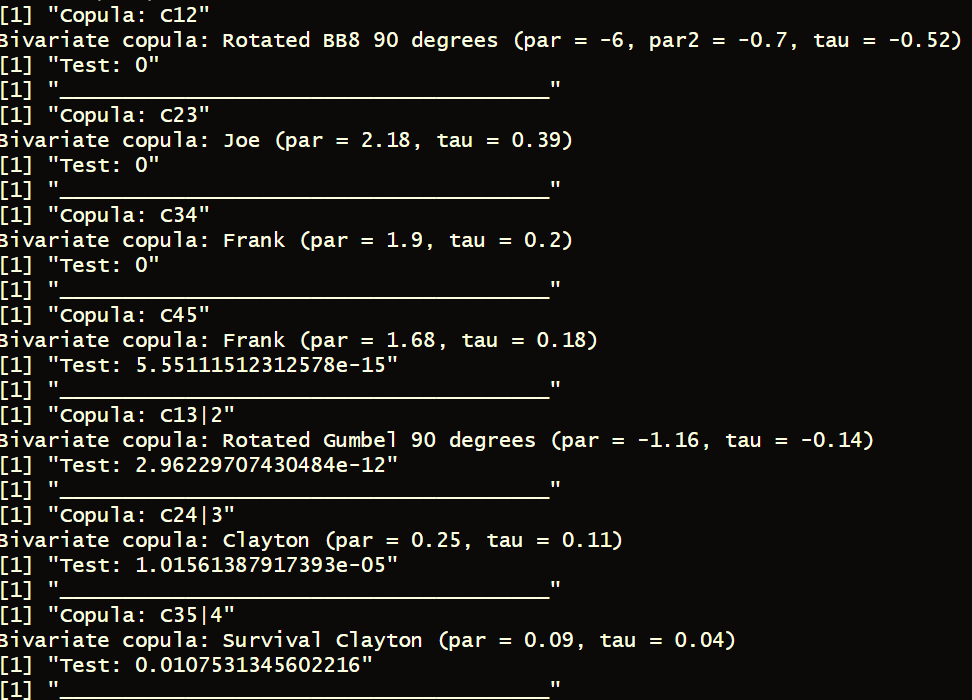
\includegraphics[width=0.46\textwidth]{4img/testM1.png}}
  \subfloat[Parte 2]{
   \label{ajusteMu2}
    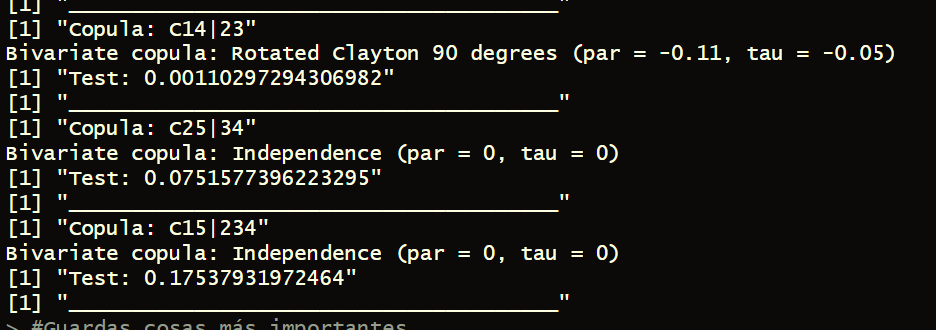
\includegraphics[width=0.46\textwidth]{4img/testM2.png}}
    \caption{Cópulas ajustadas la base de mujeres.}
    \label{fig:copulasTestMu}
\end{figure}
\vspace{-0.3cm}

Los tests de independencia de las cópulas ajustadas a los datos de mujeres que se muestran en la Figura \ref{fig:copulasTestMu}. Se puede observar en los niveles más bajos, como $C_{25|34}$ y $C_{15|234}$, muestran valores altos. Esto sugiere que podría ser beneficioso reducir una variable en estos niveles para mejorar la capacidad del modelo para capturar las relaciones entre las covariables. Los $p-valores$ relativamente altos para el test de independencia indican que las variables incluidas en estos pares de cópulas podrían no estar contribuyendo significativamente a la relación modelada. Por lo tanto, considerar la eliminación de una variable en estos niveles podría simplificar el modelo sin perder información importante sobre la dependencia entre las variables.

\begin{figure}[H]
 \centering
  \subfloat[Parte 1]{
   \label{ajusteHo1}
    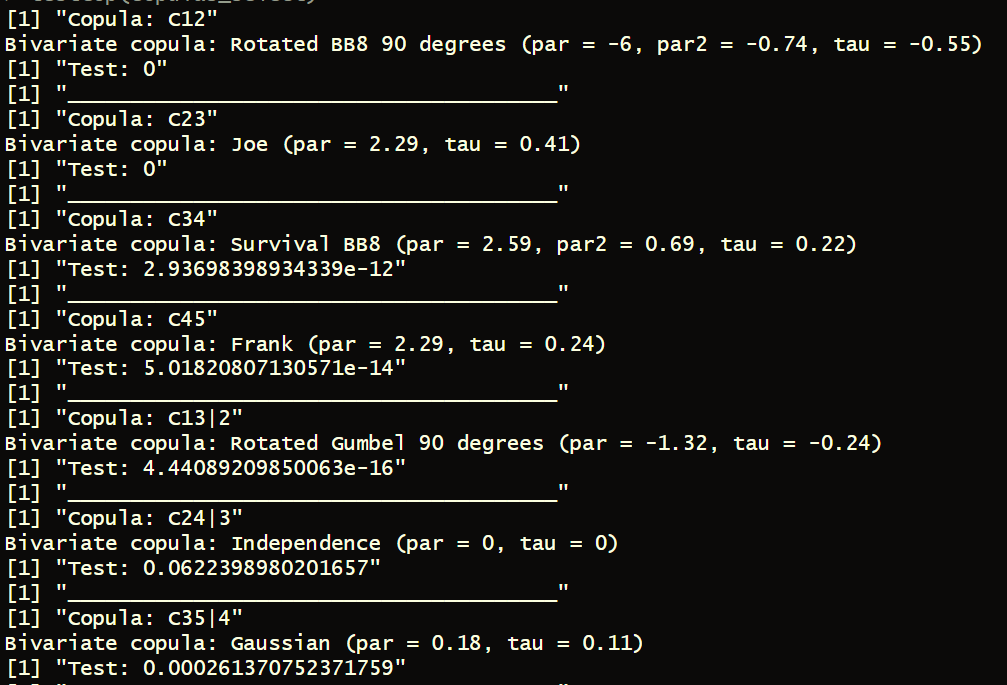
\includegraphics[width=0.46\textwidth]{4img/testH1.png}}
  \subfloat[Parte 2]{
   \label{ajusteHo2}
    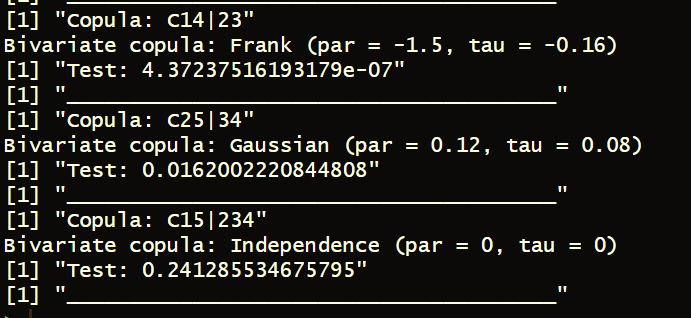
\includegraphics[width=0.46\textwidth]{4img/testH2.png}}
    \caption{Cópulas ajustadas la base de hombres.}
    \label{fig:copulasTestHo}
\end{figure}
\vspace{-0.3cm}

En cuanto a los tests de independencia de las cópulas ajustadas a los datos provenientes de hombres, ver Figura \ref{fig:copulasTestHo}, se observan $p-valores$ relativamente altos en los tests de independencia para las cópulas $C_{24|3}$ y $C_{15|234}$. Al igual que en el caso de la Figura \ref{fig:copulasTestMu}, esto sugiere que reducir una variable en estos niveles podría ser beneficioso para mejorar la capacidad del modelo para capturar las relaciones entre las covariables. 

\begin{figure}[H]
 \centering
  \subfloat[Parte 1]{
   \label{ajusteTo1}
    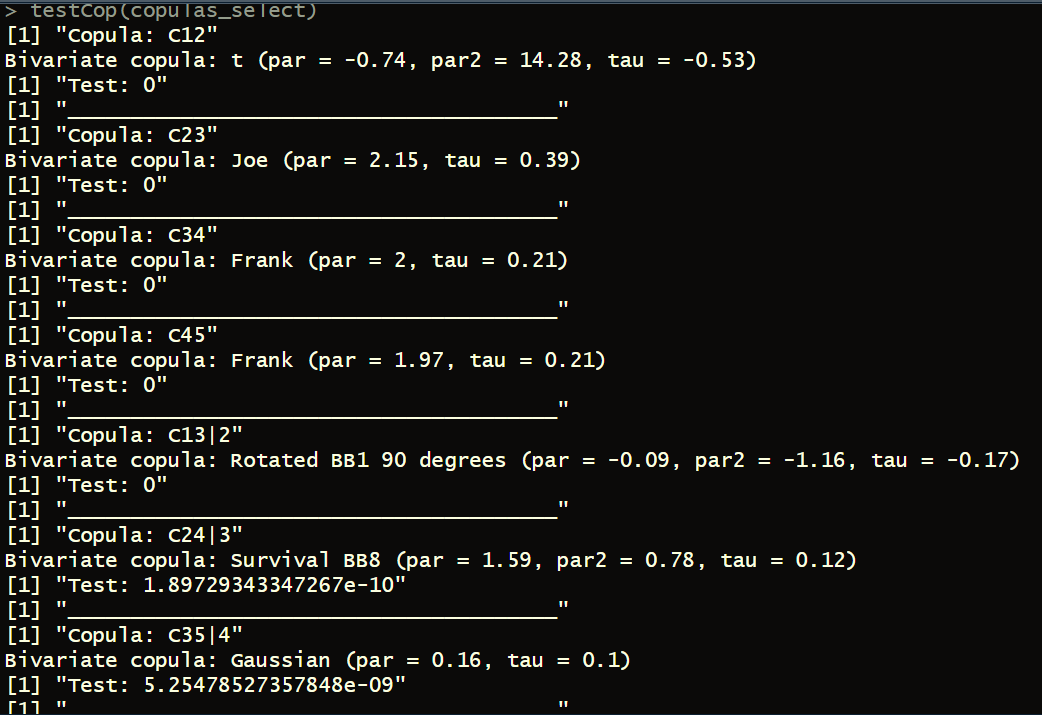
\includegraphics[width=0.46\textwidth]{4img/testT1.png}}
  \subfloat[Parte 2]{
   \label{ajusteTo2}
    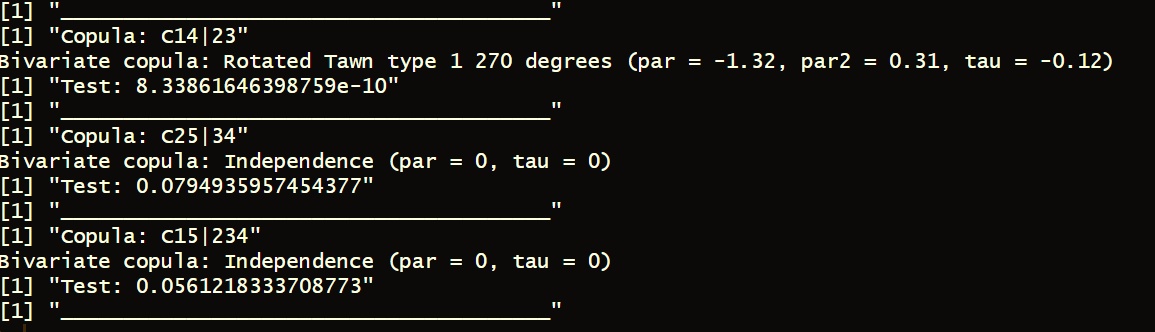
\includegraphics[width=0.46\textwidth]{4img/testT2.png}}
    \caption{Cópulas ajustadas la base de hombre y mujeres.}
    \label{fig:copulasTestTotal}
\end{figure}
\vspace{-0.3cm}

Por último, en la Figura \ref{fig:copulasTestTotal}
, se muestran las cópulas ajustadas para todo el conjunto de datos. La única cópula cuyo $p-valor$ para el test de independencia supera el nivel de confianza de $\alpha = 0.05$ es $C_{15|234}$. Es posible que esta diferencia, de solo tener una cópula independiente, se deba a que la cantidad de datos en este modelo es mayor. Al tener más datos, el modelo tiene una mayor capacidad para capturar la complejidad de las relaciones entre las variables, lo que puede resultar en una menor dependencia observada entre ellas.